\documentclass[11pt]{amsart}
\usepackage[margin=1.2in]{geometry}
\usepackage{amsmath,amssymb,amsthm,mathtools}
\usepackage{mathrsfs}
\usepackage{booktabs}
\usepackage{xcolor}
\usepackage{tikz}
\usepackage[colorlinks=true,linkcolor=blue!60!black,citecolor=blue!60!black,urlcolor=blue!60!black]{hyperref}
\usepackage{xurl}
\emergencystretch=1.5em

% ------------------------------------------------------------------ RELQ switch
% \relqclosedtrue  : RELQ proved (current state).  Title "... Sextic Orbit";
%                    the three conclusions merge in Theorem 1.1 and
%                    Section 12.2 carries the exact-model proof.
% \relqclosedfalse : RELQ open.  Title "... Six-Point Orbit"; the sextic is
%                    an exact candidate with a proved characteristic-13
%                    binding, and Theorem 1.1(3) is conditional.
\newif\ifrelqclosed
\relqclosedtrue

% ------------------------------------------------------------------ macros
\newcommand{\QQ}{\mathbb{Q}}
\newcommand{\ZZ}{\mathbb{Z}}
\newcommand{\FF}{\mathbb{F}}
\newcommand{\PP}{\mathbb{P}}
\newcommand{\GQ}{G_{\QQ}}
\newcommand{\Mtw}{M_{23}}
\newcommand{\sqm}{\sqrt{-23}}
\newcommand{\kap}{\kappa}
\newcommand{\Ni}{\operatorname{Ni}}
\newcommand{\Frob}{\operatorname{Frob}}
\newcommand{\Spec}{\operatorname{Spec}}
\newcommand{\Gal}{\operatorname{Gal}}
\newcommand{\disc}{\operatorname{disc}}
\newcommand{\Res}{\operatorname{Res}}
\newcommand{\Aut}{\operatorname{Aut}}
\newcommand{\Out}{\operatorname{Out}}
\newcommand{\Tr}{\operatorname{Tr}}
\newcommand{\Hs}{\mathscr H}
\newcommand{\xH}{x_{\mathrm H}}
\newcommand{\Cc}{\mathbf C}
\newcommand{\Garith}{G_{\mathrm{arith}}}
\newcommand{\Ggeom}{G_{\mathrm{geom}}}
\newcommand{\gU}{g_U}
\newcommand{\sextic}{x^6-x^5-3x^4-3x^3+x^2+5x+4}
\newcommand{\pp}{\mathfrak p}
\newcommand{\Xs}{\mathscr X}
\newcommand{\artifactsdoi}{10.5281/zenodo.XXXXXXXX}   % fill in before release

\theoremstyle{plain}
\newtheorem{theorem}{Theorem}[section]
\newtheorem{proposition}[theorem]{Proposition}
\newtheorem{lemma}[theorem]{Lemma}
\newtheorem{corollary}[theorem]{Corollary}
\newtheorem{conjecture}[theorem]{Conjectural identification}
\theoremstyle{definition}
\newtheorem{definition}[theorem]{Definition}
\newtheorem{remark}[theorem]{Remark}
\newtheorem{observation}[theorem]{Observation}

\ifrelqclosed
\title{The Harmonic Sheet and the Sextic Orbit}
\else
\title{The Harmonic Sheet and the Six-Point Orbit}
\fi
\ifrelqclosed
\hypersetup{pdftitle={The Harmonic Sheet and the Sextic Orbit}}
\else
\hypersetup{pdftitle={The Harmonic Sheet and the Six-Point Orbit}}
\fi
\hypersetup{pdfauthor={Alexander West Templeton},
  pdfsubject={Arithmetic and stable reduction of the seven M23 Hurwitz points}}
\author{Alexander West Templeton}
\address{Independent researcher. ORCID 0009-0005-7058-3912}
\email{alex@templeton.cloud}
\date{October 2026}

\begin{document}

\begin{abstract}
Huang, Jackson, Lee, Poonen, Pries, and Zhang realize $\Mtw$ over $\QQ$
by a rational point in the seven-point Hurwitz fiber of covers of type
$(2A,23A,23B)$. We determine the arithmetic of the fiber and the
geometry of the rational point.

At the good prime $13$ we construct an exact cover in characteristic
$13$ with geometric monodromy $\Mtw$, ordered inertia classes
$(2A,23A,23B)$ and field of moduli $\FF_{13^6}$, and show that the tame
Hurwitz problem extends to a finite \'etale scheme of rank seven over
$\ZZ_{13}$. Hence $H\simeq\Spec\QQ\sqcup\Spec E$ with $[E:\QQ]=6$: the
six nonrational covers form one Galois orbit, in which $13$ is inert.

At the bad prime $23$ we determine the stable reduction of the rational
cover. It is harmonic: the tame point, the two wild points and the
attachment point of the unique new tail are $0,\pm1,\infty$ on the
original component, the tails have conductors $7$ and $15$, and the
deformation datum is $c\,z^6dz/(z^{22}-1)$ on $z^{11}=t$, the square
class of $c$ recording the classes $23A$, $23B$. One nonsquare
cyclotomic character reverses the line and exchanges the classes, and
the harmonic datum has one lift per ordered class vector.

\ifrelqclosed
A descended Petri invariant names the orbit. An exact canonical model
of one of the six covers over $F(\sqm)$, $F=\QQ[x]/(\sextic)$,
reconstructed from the $13$-adic lift of the characteristic-$13$ point
and then verified over that field --- including an exact certificate
that its degree-$23$ map has exactly three branch points --- gives a
point of the Hurwitz scheme at which the invariant has minimal
polynomial the recognized sextic.
Hence $E\simeq F$, whose Galois closure has group $S_6$ and
discriminant $2^4\cdot11\cdot23^4$.
\else
A descended Petri invariant proposes $\QQ[x]/(\sextic)$ for $E$: the
reduction of the proposed polynomial modulo $13$ is the exact minimal
polynomial of the invariant at the degree-six point, and the
identification over $\QQ$ is stated as one explicit obligation. The
proposed field has Galois closure of group $S_6$ and discriminant
$2^4\cdot11\cdot23^4$.
\fi

The $23$-adic argument identifies the local geometry of an
independently known rational cover. It does not infer global
rationality from local fixedness.
\end{abstract}

\maketitle

% ================================================================
\section{Introduction}\label{sec:intro}

Let $H$ be the Hurwitz scheme of $\Mtw$-covers of $\PP^1$ branched at
$0,\sqm,-\sqm$ with inertia class $2A$ over $0$, $23A$ over $\sqm$ and
$23B$ over $-\sqm$ (Section~\ref{sec:fiber}). It is a finite \'etale
$\QQ$-scheme of degree seven, and \cite{HJLPPZ} exhibit a rational
point $\xH\in H(\QQ)$. Two questions. Why do the other six points form
one Galois orbit? What distinguishes $\xH$ geometrically?

Two primes answer them, and the answers do not overlap. At $13$, a
prime of good reduction, the fiber of the tame Hurwitz scheme is one
$\FF_{13}$-point and one closed point of degree six; this lifts, and
it forces the orbit structure over $\QQ$. At $23$, the prime dividing
$|\Mtw|$ exactly once, the rational cover has bad reduction of a
special shape: its stable model has an original component whose four
distinguished points are harmonic, and this shape is rigid enough to
determine the cover among the seven once the ordered classes are fixed.

The distinction is necessary. The decomposition group at $23$ is a
proper subgroup of $\GQ$, and a point of $H$ fixed by it may lie in a
$\GQ$-orbit of any size (Section~\ref{sec:insufficient}). No $23$-adic
computation therefore proves that $\xH$ is rational; rationality is
the theorem of \cite{HJLPPZ}. What $23$ can do is identify, among the
seven, the one whose local geometry a rational point must have, and
show why the symmetry that could move it does not. What $13$ can do is
count orbits. Naming the six-point orbit as a number field is a third
matter, settled in Part~III by exhibiting one of the six covers over
$F(\sqm)$ and evaluating the invariant on it.

The harmonic answer at $23$ is this. After the rescaling
$t=T/\sqm$ the branch points are $0,\pm1$, and the stable reduction of
$\xH$ has two tails, of conductors $7$ and $15$, attached at $t=0$ and
$t=\infty$; the deformation datum on $z^{11}=t$ is
$c\,z^6dz/(z^{22}-1)$ with $c$ determined up to squares, and the
square class of $c$ is the labelling of the wild points by $23A$ and
$23B$. The nonsquare cyclotomic characters reverse the harmonic line
and exchange the two classes at once, so the ordered class vector and
the datum are preserved together, and oriented patching admits exactly
one lift per ordered class vector.

The answer at $13$ is an exact object: a genus-$4$ canonical curve
over $\FF_{13^6}$ with a degree-$23$ map to $\PP^1$ of passport
$(23,\,2^81^7,\,23)$, whose monodromy is proved to be $\Mtw$ by
reconstructing the incidence count $23\cdot77=253\cdot7$ of the Witt
design $S(4,7,23)$ from a factorization, and whose field of moduli is
exactly $\FF_{13^6}$.

The division of labor is: $23$ explains the one, $13$ proves $1+6$,
and a descended Petri function $U$, evaluated on an exact model of one
of the six, names them.

\begin{theorem}\label{thm:main}
Let $H$ be as above, $\xH$ the rational point of \cite{HJLPPZ}, and
$H=\Spec\QQ\sqcup\Spec E$ the decomposition induced by $\xH$.
\begin{enumerate}
\item The stable reduction of $\xH$ at $23$ is the harmonic special
$\Mtw$-map of Theorem~\ref{thm:datum}: original component
$\PP^1_t$ with distinguished points $0,1,-1,\infty$, deformation datum
\[
  \omega_0=c\,\frac{z^6\,dz}{z^{22}-1}\quad\text{on }z^{11}=t,\qquad
  c\in\FF_{23}^\times/(\FF_{23}^\times)^2,
\]
primitive tail $x=u^{23}-u^9+u^2$ of conductor $7$ at $t=0$, and new
tail $y^3=x^5+1$, $s=20xy(x^5-8)$, of conductor $15$ at $t=\infty$.
The harmonic datum has exactly one lift for each ordered class vector,
and $\xH$ is the unique harmonic point of $H$.
\item $E$ is a field of degree six in which $13$ is inert, of
signature $(2,2)$.
\ifrelqclosed
\item $E\simeq\QQ[x]/(\sextic)$; the Galois closure of $E$ has group
$S_6$ and $\disc E=2^4\cdot11\cdot23^4$.
\else
\item Let $U\in\QQ\times E$ be the descended Petri function of
Section~\ref{sec:petri} and $\gU$ its characteristic polynomial on
$E$. The exact value of $U$ at the degree-six point of $H_{\FF_{13}}$
generates $\FF_{13^6}$ and has minimal polynomial $\Phi\bmod13$, where
$\Phi$ is the sextic of Section~\ref{sec:petri} with
$\QQ[x]/(\Phi)\simeq\QQ[x]/(\sextic)$. If $\gU=\Phi$
(Conjectural identification~\ref{conj:relq}), then
$E\simeq\QQ[x]/(\sextic)$, the Galois closure of $E$ has group $S_6$,
and $\disc E=2^4\cdot11\cdot23^4$.
\fi
\end{enumerate}
\end{theorem}

The theorem is not proved in its displayed order. Part~I proves
assertion~2 at the good prime $13$; Part~II proves assertion~1 at the
bad prime $23$; Part~III proves the exact identification in
assertion~3, at neither prime. In one line:
\[
\boxed{\ \text{seven covers}
 =\underbrace{\text{one harmonic sheet}}_{23}
 +\underbrace{\text{one sextic orbit}}_{13,\ F(\sqm)}\ }
\]

% ================================================================
\section{The seven-point Hurwitz fiber}\label{sec:fiber}

\subsection{The ordered class problem}\label{sec:ordered}

Let $G=\Mtw$, $\Cc=(2A,23A,23B)$, $K=\QQ(\sqm)$, and
$B=\{0,\sqm,-\sqm\}\subset\PP^1$. Over $K$ the three branch points are
rational and ordered, and the Hurwitz scheme $H_K$ of $G$-covers of
$\PP^1_K$ branched at $B$ with inertia $2A$ over $0$, $23A$ over $\sqm$
and $23B$ over $-\sqm$ is a finite \'etale $K$-scheme with
\[
  H_K(\overline K)\simeq\Ni^{\mathrm{in}}(\Cc)
  =\bigl\{(x,y,z)\in 2A\times23A\times23B:\ xyz=1,\
  \langle x,y\rangle=\Mtw\bigr\}/\Mtw ,
\]
a set of seven elements \cite{HJLPPZ,seven}.

\begin{proposition}\label{prop:descent}
\begin{enumerate}
\item $H_K$ descends to a finite \'etale $\QQ$-scheme $H$ of degree
seven.
\item $H$ is a fine moduli scheme for $G$-covers in the class, and the
residue field of a closed point is the field of moduli of the
corresponding cover.
\item For a cover $Y$ in the class, the degree-$23$ quotient
$X=Y/M_{22}\to\PP^1$ has no nontrivial automorphism over $\PP^1$, its
Galois closure is $Y$, and it has a unique point over each of $\pm\sqm$.
\end{enumerate}
\end{proposition}
\begin{proof}
(1) Since $23\equiv3\pmod4$, $K$ is the quadratic subfield of
$\QQ(\zeta_{23})$, so $\sigma\in\GQ$ swaps $\pm\sqm$ exactly when
$\chi_{23}(\sigma)$ is a nonsquare modulo $23$. The same $\sigma$ acts
on the classes of order $23$ by $y\mapsto y^{\chi_{23}(\sigma)}$, and
$y^k\sim y$ in $\Mtw$ iff $k$ is a square modulo $23$
\cite{ATLAS}, so it swaps $23A$ and $23B$. The assignment of classes to
branch points is therefore $\GQ$-equivariant, and it defines a descent
datum for $H_K$ over $\QQ$.
(2) $Z(\Mtw)=1$, so a $G$-cover in the class has no automorphisms
commuting with $G$; the Hurwitz functor of $G$-covers with prescribed
inertia is then representable \cite{Fulton,RomagnyWewers}, and the
residue field of a point is the field of moduli of its cover, which
for $Z(G)=1$ is also a field of definition \cite{DebesDouai}.
(3) $M_{22}$ is maximal and not normal in the simple group $\Mtw$,
hence self-normalizing, so $\Aut(X/\PP^1)=N_G(M_{22})/M_{22}=1$; it is
core-free, so the Galois closure of $X\to\PP^1$ is $Y$. A point over
a totally ramified branch point is unique in its fiber.
\end{proof}

\subsection{The rational point and complex conjugation}

\cite{HJLPPZ} exhibit $\xH\in H(\QQ)$, the class of their printed
triple; in the numbering of \cite{seven} it is label $6$. Complex
conjugation acts on the seven as $\kap=(1\,2)(5\,7)$ \cite[Thm.~3.1]{seven}: it
fixes $\xH$ and two other points and swaps two pairs. Write
$H=\Spec A$ with $A$ an \'etale $\QQ$-algebra of degree seven. The
rational point splits off an idempotent:
\[
  H=\Spec\QQ\sqcup\Spec E,\qquad \dim_\QQ E=6 .
\]

\subsection{Why local fixedness is insufficient}\label{sec:insufficient}

The point $\xH$ is fixed by every decomposition group, in particular
by $D_{23}$. Nothing follows from this alone: the septic
$x^7-x-1$ is irreducible with Galois group $S_7$ \cite{Osada}, and it
factors as a linear times an irreducible sextic both modulo $23$ and
modulo $13$; so $\Spec\QQ[x]/(x^7-x-1)$ has a unique $\QQ_{23}$-point
and fiber shape $1+6$ at $13$, yet its seven geometric points form a
single $\GQ$-orbit. In Part~I the global input is the rational point
$\xH$, which splits $E$ off as a six-dimensional algebra; the prime
$13$ then shows that $E$ is a field. In Part~II the existence of a
rational point is again the input, from \cite{HJLPPZ}; the prime $23$
identifies which point it is and why its local structure is rigid.
Neither argument substitutes for the other.

% ================================================================
\part{Six: arithmetic at 13}

\section{The tame Hurwitz model}\label{sec:model}

Since $-23\equiv4^2\pmod{13}$, the prime $13$ splits in $K$; fix the
place with $\sqm\mapsto s\in\ZZ_{13}$, $s\equiv4\pmod{13}$. The three
sections $0,s,-s$ of $\PP^1_{\ZZ_{13}}$ are pairwise disjoint.

\begin{lemma}\label{lem:model}
There is a finite \'etale $\ZZ_{13}$-scheme $\Hs$ of rank seven with
generic fiber $H\otimes\QQ_{13}$, whose points over an algebraically
closed field $k$ of characteristic $13$ are the isomorphism classes of
tame $\Mtw$-covers of $\PP^1_k$ branched exactly over $0,s,-s$ with
inertia classes $2A,23A,23B$ respectively.
\end{lemma}
\begin{proof}
$13\nmid|\Mtw|=2^7\cdot3^2\cdot5\cdot7\cdot11\cdot23$, so every cover
in question is tame. The Hurwitz stack of tame $G$-covers of $\PP^1$
branched along disjoint sections with prescribed inertia classes is
finite \'etale over the base \cite{Fulton,RomagnyWewers}, and it is
representable because $Z(G)=1$. Its geometric fibers are the Nielsen
classes, of seven elements in every characteristic prime to $|G|$:
tame specialization is a bijection on inertia-marked Nielsen classes.
\end{proof}

$\Frob_{13}$ fixes $0,\pm s$ and, since $13\equiv6^2\pmod{23}$, fixes
the classes $23A$ and $23B$. As $\Hs$ is finite over $\ZZ_{13}$,
$\Hs(\QQ_{13})=\Hs(\ZZ_{13})$, and $\xH$ reduces to a point
$\bar x_{\mathrm H}\in\Hs(\FF_{13})$.

% ================================================================
\section{The exact degree-six point}\label{sec:point}

\subsection{Canonical curve and degree-23 map}

Let $k=\FF_{13}[a]/(a^6+12a^5+10a^4+10a^3+a^2+5a+4)=\FF_{13^6}$; the
modulus is the reduction of the sextic of Section~\ref{sec:petri}. In
\cite[petri-f13]{receipts} an exact smooth genus-$4$ canonical curve
$X=V(Q,C)\subset\PP^3_k$ is constructed, $Q$ a quadric and $C$ a
cubic (Appendix~\ref{app:model}), together with a map
\[
  t=N/D\colon X\to\PP^1,\qquad \deg t=23,
\]
$N,D$ quintic forms with $\operatorname{div}(t)=23P_0-23P_\infty$,
$P_0=(1{:}0{:}0{:}0)$. Let $\lambda\in k$ be the third branch value,
put $\tau=\lambda/t$, so that $\tau$ has branch points $\infty,1,0$
over $P_0$, the $\lambda$-fiber and $P_\infty$, and write $Q:=P_0$.

\begin{proposition}\label{prop:passport}
The cover $\tau\colon X\to\PP^1$ is tame with passport
$(23,\ 2^81^7,\ 23)$: totally ramified over $\infty$ and $0$, and over
$1$ eight places with $e=2$ and seven with $e=1$.
\end{proposition}
\begin{proof}
The fiber over $t=\lambda$ is a scheme of degree $23$ with reduced
degree $15=7+8$ (Appendix~\ref{app:model}). The different has degree
$2g-2+2\cdot23=52=22+22+8$, so exactly the eight double points ramify,
each with $e=2$, and there is no further ramification.
\end{proof}

\subsection{Ordinary ramification points}

\begin{proposition}\label{prop:gaps}
The Weierstrass gap sequence at $Q$ and at $P_\infty$ is $(1,2,3,4)$;
the first nongap is $5$. In particular both totally ramified points are
ordinary points of $X$.
\end{proposition}
\begin{proof}
The order sequence of the canonical system at each point is
$(0,1,2,3)$, read off the exact local expansions of the canonical
coordinates by row reduction (Appendix~\ref{app:model}); the order
sequences of $|2K_X|$ and $|3K_X|$ confirm the semigroup
$\{0\}\cup[5,\infty)$.
\end{proof}

\subsection{The low-pole coordinate}

Since $5$ is the first nongap, $L(5Q)=k\oplus k\,u'$. Let $w$ be the
uniformizer at $Q$ with $\tau=w^{-23}$, unique because
$\gcd(23,13^6-1)=1$, and normalize $u'=w^{-5}+O(w^{-4})$,
$\Tr_{k(\tau)}u'=0$; this fixes $u'$.

\begin{lemma}\label{lem:hprime}
$u'$ generates $k(X)$ over $k(\tau)$. Its minimal polynomial
\[
  H'(\tau,U)=U^{23}+\sum_{i\ge5}c_i(\tau)\,U^{23-i}\in k[\tau][U]
\]
has $\deg_\tau c_i\le\lfloor5i/23\rfloor$, $H'(0,U)=U^{23}$, and
$H'(1,U)=q_7'\,d_8'^{\,2}$ with $q_7'$, $d_8'$ squarefree and coprime
of degrees $7$ and $8$.
\end{lemma}
\begin{proof}
$[k(X):k(\tau,u')]$ divides the prime $23$, and $u'\notin k(\tau)$
because nonconstant elements of $k(\tau)$ have degree divisible by
$23$ on $X$ while $u'$ has degree $5$. The degree bounds are the
valuation bounds at $Q$, the constant term is $\tau=\infty$ at $Q$,
and the shape at $\tau=1$ is the passport. $H'$ is computed twice,
by a linear solve on the $w$-expansion and by Gr\"obner elimination
(Appendix~\ref{app:model}).
\end{proof}

% ================================================================
\section{The Witt incidence certificate}\label{sec:witt}

Let $F=k(X)$, $L$ its Galois closure over $k(\tau)$, and
\[
  \Garith=\Gal(L/k(\tau)),\qquad
  \Ggeom=\Gal(L\bar k/\bar k(\tau)) ,
\]
the arithmetic and geometric monodromy groups, both acting on the
$23$ roots of $H'$. Since $X$ is geometrically irreducible, $\Ggeom$
is transitive; it is identified with $\Gal(L/k'(\tau))$, $k'=L\cap\bar
k$, a normal subgroup of $\Garith$ with cyclic quotient $\Gal(k'/k)$.

Over the completion at $Q$ the roots of $H'$ are $u'(\zeta^jw)$,
$j\in\ZZ/23$, for a primitive $23$rd root of unity $\zeta$, so
$7$-subsets of roots are $7$-subsets of $\ZZ/23$. Let $\mathcal D$ be
the cyclic Steiner system $S(4,7,23)$ on $\ZZ/23$ with base block
$\{0,1,2,3,9,12,21\}$ (Appendix~\ref{app:heptad}; the other cyclic
$S(4,7,23)$ is its nonsquare twist $\mathcal D'=5\mathcal D$), and
form the block resolvent
\[
  \Theta(Y)=\prod_{B\in\mathcal D}\bigl(Y-\theta_B\bigr),\qquad
  \theta_B=\sum_{i\in B}u'(\zeta^iw),
\]
a monic polynomial of degree $253$ whose coefficients are a priori
Laurent series in $w$ over $\FF_{13^{66}}=k(\zeta)$.

\begin{proposition}\label{prop:theta}
$\Theta\in k[\tau][Y]$, with the coefficient of $Y^{253-i}$ of degree
$\le\lfloor5i/23\rfloor$ in $\tau$, and $\Theta$ is irreducible over
$k(\tau)$.
\end{proposition}
\begin{proof}
Appendix~\ref{app:heptad}: the coefficients are computed as series to
relative precision $O(w^{1450})$ and are polynomials in $\tau=w^{-23}$
within the stated bounds; irreducibility holds already over
$k((\tau^{-1}))$, because the $253$ roots are simple modulo $w$ after
$Y\mapsto w^{-5}Y$ and the local Galois group permutes them
transitively.
\end{proof}

\begin{proposition}\label{prop:factor}
Let $\Psi_{77}$ be the product over the $77$ blocks containing $0$ and
$\Psi_{176}$ the product over the other $176$. Then $\Psi_{77}$ and
$\Psi_{176}$ lie in $F[Y]$, and
\[
  \Theta=\Psi_{77}\,\Psi_{176}\quad\text{in }F[Y].
\]
\end{proposition}
\begin{proof}
Appendix~\ref{app:heptad}: each coefficient of $\Psi_{77}$ and
$\Psi_{176}$ is matched against the pole-order basis of
$\mathcal O_Q=\bigcup_mL(mQ)$; the matching vanishes at the gap
orders, and the difference $\Psi_{77}\Psi_{176}-\Theta$ has
coefficients with poles only at $Q$ and positive valuation there,
hence zero.
\end{proof}

\begin{theorem}\label{thm:mon13}
$\Garith=\Mtw$ and $\Ggeom=\Mtw$.
\end{theorem}
\begin{proof}
$\Garith$ is transitive of prime degree, hence primitive. The inertia
over $\tau=1$ contains an element of cycle type $2^81^7$
(Proposition~\ref{prop:passport}), an even permutation with seven
fixed points; no affine group of degree $23$ contains such an element,
so by the classification of primitive groups of degree $23$,
$\Garith\in\{\Mtw,A_{23},S_{23}\}$.

The roots of $\Theta$ are sums of roots of $H'$, so $\Theta$ splits
in $L$ and $\Garith$ acts on its $253$ roots, transitively by
Proposition~\ref{prop:theta}. By Proposition~\ref{prop:factor} the
$77$ roots of $\Psi_{77}$ form a set stable under the stabilizer of
$u'$, so the $\Garith$-orbit $R$ of
$\{u'\}\times\operatorname{roots}(\Psi_{77})$ inside
$\operatorname{roots}(H')\times\operatorname{roots}(\Theta)$ has
fibers of size $77$ over each root of $H'$:
\[
  |R|=23\cdot77=1771=253\cdot7 .
\]
By transitivity on the roots of $\Theta$, every fiber $R_\beta$ over
a root $\beta$ of $\Theta$ has exactly $7$ elements. The map
$\beta\mapsto R_\beta$ is $\Garith$-equivariant, so its image is a
single $\Garith$-orbit of $7$-subsets of the roots of $H'$, of size at
most $253$. But $A_{23}$ and $S_{23}$ are transitive on $7$-subsets,
with orbit size $\binom{23}{7}=245157$. Hence $\Garith=\Mtw$.

$\Ggeom$ is a transitive normal subgroup of the simple group $\Mtw$,
so $\Ggeom=\Mtw$.
\end{proof}

\begin{proposition}[orientation]\label{prop:orient}
The inertia generators at $Q$ and at $P_\infty$ lie in different
$\Mtw$-classes of elements of order $23$. With the involution over
$\tau=1$ in the unique class $2A$, the ordered class vector of the
cover is $(2A,23A,23B)$ up to the choice of which totally ramified
point is called $23A$.
\end{proposition}
\begin{proof}
At $P_\infty$, $\tau=w'^{23}$ for the exact uniformizer $w'$, and the
roots of $H'$ are $u'(\zeta^jw')$ with the same $\zeta$. The block sums
of the twisted design $\mathcal D'$, not of $\mathcal D$, reproduce
$\Theta(w'^{23},Y)$ (Appendix~\ref{app:heptad}). Transporting the
$P_\infty$-labelling to the $Q$-labelling therefore composes the
inertia generator with the multiplier $5$, a nonsquare modulo $23$,
and $y^k\sim y$ in $\Mtw$ only for square $k$.
\end{proof}

The identity $23\cdot77=253\cdot7$ is the incidence count of points
and blocks of $S(4,7,23)$, reconstructed from a factorization rather
than assumed; $A_{23}$ would give $22+231$ in place of $77+176$. The
same certificate will settle the tails at $23$
(Proposition~\ref{prop:tailmon}).

% ================================================================
\section{One plus six}\label{sec:onesix}

\begin{lemma}\label{lem:moduli}
The cover $\tau\colon X\to\PP^1$ with its inertia labelling defines a
closed point of $\Hs_{\FF_{13}}$ with residue field $\FF_{13^6}$.
\end{lemma}
\begin{proof}
The three branch points carry three distinct classes, so the M\"obius
transformation sending them, in the order $(2A,23A,23B)$, to $(0,s,-s)$
modulo $13$ is unique, and it is defined over $k$ because $0,\pm s$
are $\FF_{13}$-rational: the labelled cover is a $k$-point of $\Hs$.
Its Frobenius conjugates are labelled covers with the same labels, and
the normalized data $(\tau,Q,w,u')$ is a function of the labelled
isomorphism class, so $\Frob^d$ fixes the point iff it fixes the
coefficients of $H'$. The smallest such $d$ is $6$
(Appendix~\ref{app:model}).
\end{proof}

\begin{theorem}\label{thm:onesix}
\[
  \boxed{\ \Hs_{\FF_{13}}\simeq\Spec\FF_{13}\sqcup\Spec\FF_{13^6}\ }
\]
Consequently $E$ is a field of degree six in which $13$ is inert, with
signature $(2,2)$: $\GQ$ acts transitively on the six nonrational
points, $\Frob_{13}$ as a $6$-cycle and complex conjugation as a
double transposition.
\end{theorem}
\begin{proof}
$\Hs_{\FF_{13}}$ has rank seven and contains the $\FF_{13}$-point
$\bar x_{\mathrm H}$ and the degree-six closed point of
Lemma~\ref{lem:moduli}; $1+6=7$ gives the display. Idempotents of a
finite \'etale algebra over the henselian ring $\ZZ_{13}$ lift
uniquely from the special fiber, so
$\Hs=\Spec\ZZ_{13}\sqcup\Spec\mathcal O$ with $\mathcal O$ the
unramified sextic extension of $\ZZ_{13}$. Comparing with
$H\otimes\QQ_{13}=\QQ_{13}\times(E\otimes\QQ_{13})$, the component
containing $\xH$ is $\Spec\ZZ_{13}$, so
$E\otimes\QQ_{13}=\mathcal O\otimes\QQ$ is a field: $E$ is a field and
$13$ is inert. The signature is read off $\kap$, which fixes two of
the six and swaps two pairs.
\end{proof}

This proves assertion~2 of Theorem~\ref{thm:main}. No
stable-reduction formula has been used.

% ================================================================
\part{One: harmonic reduction at 23}

\section{The harmonic component}\label{sec:collision}

\subsection{Collision and the exceptional line}

In the coordinate $T$ of \cite{HJLPPZ} the three branch points are
$0,\sqm,-\sqm$; modulo a prime above $23$ they collide. The collision
is a property of the coordinate, not of the configuration: after the
rescaling
\[
  t=T/\sqm
\]
the branch points are $0,1,-1$, and the configuration has good
reduction. What is bad at $23$ is the cover, whose two inertia groups
of order $23$ are wild. In the stable model the $t$-line is the
\emph{original component} $\bar X_0$ of \cite{Wewers}; it carries the
two wild points $t=\pm1$, the primitive tail containing the tame point
attaches at $t=0$, and the unique new tail (Section~\ref{sec:newtail})
attaches at $t=\infty$. So $\bar X_0$ has four distinguished points
$0,1,-1,\infty$, of cross-ratio $-1$ (Figure~\ref{fig:stable}).

\begin{figure}[t]
\centering
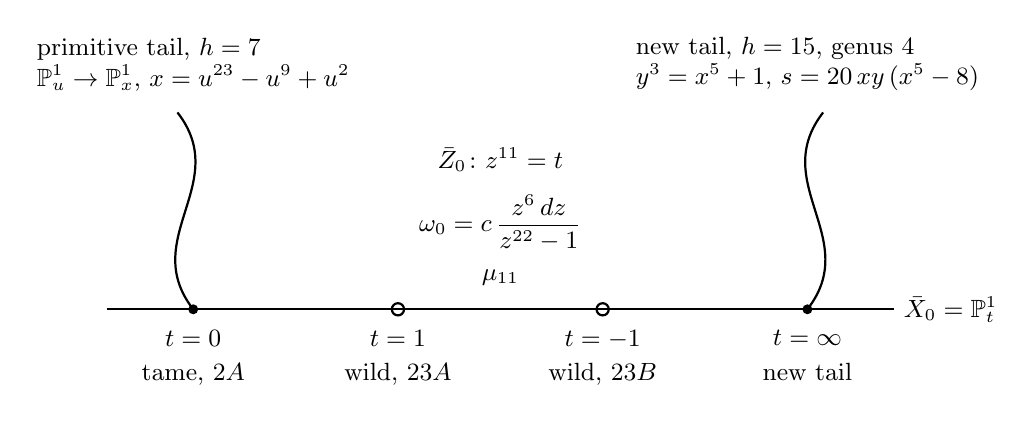
\begin{tikzpicture}[scale=1.0, every node/.style={font=\small}]
  % original component
  \draw[thick] (-5.0,0) -- (5.0,0);
  \node[right] at (5.0,0) {$\bar X_0=\PP^1_t$};
  % marked points
  \fill (-3.9,0) circle (1.8pt);
  \node[below=4pt] at (-3.9,0) {$t=0$};
  \node[below=16pt] at (-3.9,0) {tame, $2A$};
  \draw[thick] (-1.3,0) circle (2.2pt);
  \node[below=4pt] at (-1.3,0) {$t=1$};
  \node[below=16pt] at (-1.3,0) {wild, $23A$};
  \draw[thick] (1.3,0) circle (2.2pt);
  \node[below=4pt] at (1.3,0) {$t=-1$};
  \node[below=16pt] at (1.3,0) {wild, $23B$};
  \fill (3.9,0) circle (1.8pt);
  \node[below=4pt] at (3.9,0) {$t=\infty$};
  \node[below=16pt] at (3.9,0) {new tail};
  % primitive tail at t=0 (a curve leaving the line)
  \draw[thick] (-3.9,0) .. controls (-4.6,0.9) and (-3.4,1.6) .. (-4.1,2.5);
  \node[align=left,anchor=south] at (-3.9,2.65)
    {primitive tail, $h=7$\\ $\PP^1_u\to\PP^1_x$, $x=u^{23}-u^9+u^2$};
  % new tail at t=infinity
  \draw[thick] (3.9,0) .. controls (4.6,0.9) and (3.4,1.6) .. (4.1,2.5);
  \node[align=left,anchor=south] at (3.9,2.65)
    {new tail, $h=15$, genus $4$\\ $y^3=x^5+1$, $s=20\,xy\,(x^5-8)$};
  % datum
  \node at (0,1.9) {$\bar Z_0\colon z^{11}=t$};
  \node at (0,1.1) {$\omega_0=c\,\dfrac{z^6\,dz}{z^{22}-1}$};
  \node at (0,0.4) {$\mu_{11}$};
\end{tikzpicture}
\caption{The stable reduction of $\xH$ at $23$ (Theorem~\ref{thm:harmonic}).
Filled points are tail attachments, open points are the wild branch
points; the cross-ratio of $0,1,-1,\infty$ is $-1$. The datum lives
on the $\mu_{11}$-cover $\bar Z_0\to\bar X_0$.}
\label{fig:stable}
\end{figure}

\begin{definition}\label{def:harmonic}
A special $\Mtw$-map at $23$ in the sense of \cite{Wewers} is
\emph{harmonic} if the four distinguished points of its original
component --- the tame attachment point, the two wild points, and the
attachment point of the new tail --- form a harmonic quadruple, i.e.\
are $0,\pm1,\infty$ in a suitable coordinate. A point of $H$ is
harmonic if its stable reduction at $23$ is harmonic.
\end{definition}

We use the following facts from \cite{Wewers}, for a three-point
$G$-cover with $p\,\|\,|G|$ and bad reduction at $p=23$. The stable
model has an original component with a special deformation datum
$(\bar Z_0,\omega_0)$, where $\bar Z_0\to\bar X_0$ is the
$\mu_m$-cover with $m=|N_G(P)/C_G(P)|$, $P$ a Sylow $23$-subgroup;
here $N_{\Mtw}(P)=23{:}11$, so $m=11$ and $\bar Z_0\colon z^{11}=t$.
Every other component is a tail with a conductor $h_j$; the primitive
tail contains the tame branch point, the new tails contain no branch
point, and the vanishing-cycle relation reads
\[
  h_{\mathrm{prim}}+\sum_{\text{new}}(h_j-11)=11 .
\]

\subsection{The primitive tail}\label{sec:primtail}

\begin{proposition}\label{prop:prim}
The primitive tail of $\xH$ is $\PP^1_u\to\PP^1_x$,
\[
  x=u^{23}-u^9+u^2=u^2(u^7+10)^2(u^7+3),
\]
with the tame point at $x=0$ (fiber $2^81^7$), the wild point at
$u=\infty$, and conductor $h_{\mathrm{prim}}=7$.
\end{proposition}
\begin{proof}
The exact model $F(V,T)$ of \cite{HJLPPZ} has, at a double point of
$F(V,0)$, a Newton facet that becomes visible under the scaling
$(V,T)\mapsto(23^{1/7}V,\,23^{15/7}T)$; the facet polynomial is
$13Z^2+12WZ+W^2(1+W^7+2W^{14}+W^{21})$, rational with $W=w^2$,
$Z=A(w^{23}+w^9)+19w^2$, $A^2=7$, which is the displayed map over
$\FF_{23}$. The conductor is read off Riemann--Hurwitz: the degree-$23$
map $\PP^1\to\PP^1$ has different of degree $44$, of which $8$ is tame
at $x=0$, so the wild point has different exponent
$36=(p-1)(1+h/m)$ with $m=11$, $h=7$.
\end{proof}

\begin{proposition}\label{prop:primunique}
Up to isomorphism, $x=u^{23}-u^9+u^2$ is the only tail cover with a
tame point of type $2^81^7$ and conductor $7$, and its automorphism
group over the base is $\mu_7$.
\end{proposition}
\begin{proof}
Appendix~\ref{app:infinity}: writing $x=P(u)$ with $P'=9q$, $P=q^2r$
gives a zero-dimensional system with $429$ solutions, all
equivalent to the displayed one under the affine normalizations.
\end{proof}

% ================================================================
\section{The infinity tail}\label{sec:newtail}

Write $G(V,S)=(1+23S^2)^4F(V,1/S)$ for the model at $T=\infty$. Its
reduction at $S=0$ is $(V+5)^{23}$: one inseparable center. Recenter
$V=18+W$ and let $\beta=v(S)$ vary.

\begin{proposition}[chambers]\label{prop:chambers}
The Newton polygon of $G(18+W,S)$ in $W$ has exactly one change of
lower hull as $\beta$ varies, at
\[
  \beta=\tfrac4{15}=\tfrac{23}{2\cdot15}-\tfrac12 ,
\]
where the single wild cluster $v(W)=(3+6\beta)/23$ first enters
$\tfrac15\ZZ$. For $\beta>4/15$ the fiber over a point of the disc
splits as $3+5+15$ with $(e,f)=(3,1),(5,1),(15,1)$: the tame inertia
of the disc is cyclic of order exactly $15$, with orbits $15,5,3$.
\end{proposition}
\begin{proof}
The exact computation has $258$ candidate breakpoints and only one
change of lower hull; the ramification indices are Ore's theorem for
the factors of degrees $3$ and $5$ and a second-order Montes step for
the factor of degree $15$ (Appendix~\ref{app:infinity}).
\end{proof}

\begin{corollary}\label{cor:hnew}
$\xH$ has exactly one new tail. It attaches at $t=\infty$, has
conductor $h_{\mathrm{new}}=15$ and genus $4$.
\end{corollary}
\begin{proof}
The tame inertia of order $15$ acts faithfully on the tail through
its automorphism group over the base, which is cyclic of order dividing
$22h$ \cite[Prop.~3.11]{Wewers}; so $15\mid h$. A new tail has
$12\le h\le21$; hence $h=15$, and the genus is $h-11=4$. The
vanishing-cycle relation $h_{\mathrm{prim}}+(h_{\mathrm{new}}-11)=7+4=11$
is exhausted, so there is no other tail.
\end{proof}

\begin{proposition}\label{prop:new}
The new tail is the genus-$4$ curve
\[
  D\colon y^3=x^5+1,\qquad s=20\,xy\,(x^5-8),
\]
with $s\colon D\to\PP^1$ of degree $23$ branched only at the wild
point $Q$ over $s=\infty$, where the different exponent is
$52=(p-1)(1+15/11)$.
\end{proposition}
\begin{proof}
Riemann--Hurwitz for the $C_{15}$-quotient with orbits of length
$15,5,3$ gives ramification $14+12+10=36=2\cdot4-2+30$, so the
quotient has genus $0$ and $D$ is the unique cyclic $15$-cover of
$\PP^1$ with these indices: $y^3=x^5+1$. The degree-$23$ map is
determined by its differential: $dx/y^2$ has divisor $6Q$, is exact in
characteristic $23$ because $dx/y^2=y^{-23}(x^5+1)^7dx$ and
$5j+1\not\equiv0$ for $j\le7$, and its primitive is unique up to
constants since $l(Q)=1$; that primitive is $s=20xy(x^5-8)$, with
$s^3=19x^3(x^5-8)^3(x^5+1)$. Its differential is $dx/y^2$ up to a
constant, so $s$ is unramified away from $Q$.
\end{proof}

\begin{proposition}\label{prop:tailmon}
Both tail covers have geometric monodromy $\Mtw$.
\end{proposition}
\begin{proof}
Each is transitive of prime degree; the primitive tail has inertia
of type $2^81^7$, and the new tail is the $\mu_3$-pullback of
$\PP^1_x\to\PP^1_{s^3}$, whose inertia over $0$ has type $3^61^5$. So
each group is $\Mtw$, $A_{23}$ or $S_{23}$. The Witt certificate of
Section~\ref{sec:witt} settles both: over $\FF_{23}(x)$ the block
resolvent $\Theta$ of degree $253$ is irreducible and factors over the
rational function field of the tail as $\Psi_{77}\Psi_{176}$
(Appendix~\ref{app:heptad}), giving $23\cdot77=253\cdot7$ again;
$D\to\PP^1_s$ then has monodromy of index dividing $3$ in $\Mtw$,
hence $\Mtw$.
\end{proof}

% ================================================================
\section{The central datum}\label{sec:datum}

\begin{theorem}\label{thm:datum}
The special deformation datum of $\xH$ at $23$ lives on
$\bar Z_0\colon z^{11}=t$ and equals
\[
  \omega_0=c\,\frac{z^6\,dz}{z^{22}-1},\qquad c\in\FF_{23}^\times,
\]
where $c$ is determined exactly up to squares.
\end{theorem}
\begin{proof}
\emph{Divisor.} The datum is a logarithmic differential on $\bar Z_0$
with simple poles exactly at the $22$ points over the wild points
$t=\pm1$, and zeros of orders determined by the conductors at the two
tail attachments: $h_{\mathrm{prim}}-1=6$ at $z=0$ and
$h_{\mathrm{new}}-1=14$ at $z=\infty$. So
\[
  \operatorname{div}\omega_0=6[0]+14[\infty]-\sum_{\eta^{22}=1}[\eta],
\]
of degree $-2$ on $\PP^1_z$; the space of such differentials is
one-dimensional, spanned by $z^6dz/(z^{22}-1)$.

\emph{Cartier.} Logarithmic means $\mathcal C(\omega_0)=\omega_0$ for
the Cartier operator. Expand at $z=0$:
$\omega_c=-c\sum_{n\ge0}z^{6+22n}\,dz$. Since
$\mathcal C(z^{e}dz)=z^{(e+1)/23-1}dz$ when $23\mid e+1$ and $0$
otherwise, only the terms with $23\mid 7+22n$, i.e.\ $n\equiv7\pmod{23}$,
survive; for $n=7+23\ell$ the exponent $e=6+22n$ has
$(e+1)/23-1=6+22\ell$, so
\[
  \mathcal C(\omega_c)=-c^{1/23}\sum_{\ell\ge0}z^{6+22\ell}\,dz=\omega_{c^{1/23}} .
\]
Thus $\omega_c$ is logarithmic iff $c^{23}=c$, i.e.\ $c\in\FF_{23}$.
The datum is defined only up to the automorphisms $z\mapsto\xi z$,
$\xi^{11}=1$, of $\bar Z_0$ over $\bar X_0$, which send $\omega_c$ to
$\omega_{c\xi^7}$; and $\{\xi^7:\xi^{11}=1\}=\mu_{11}=(\FF_{23}^\times)^2$.
So $c$ is determined exactly up to its square class.
\end{proof}

\begin{proposition}[residues]\label{prop:res}
For $\eta^{22}=1$, $\Res_{z=\eta}\omega_c=-c\,\eta^7$. Over $t=1$ the
residues fill one square class of $\FF_{23}^\times$, namely
$-c\cdot(\FF_{23}^\times)^2$; over $t=-1$ they fill the other.
\end{proposition}
\begin{proof}
$\Res_{z=\eta}=c\eta^6/(22\eta^{21})=-c\eta^{-15}=-c\eta^{7}$. Over
$t=1$ we have $\eta\in\mu_{11}$, and $\eta\mapsto\eta^7$ is a bijection
of $\mu_{11}=(\FF_{23}^\times)^2$. Over $t=-1$, $\eta=-\xi$ with
$\xi\in\mu_{11}$, and $(-\xi)^7=-\xi^7$ runs through the nonsquares.
\end{proof}

The residue of the datum at a wild point is the character of the
tame part of inertia there, and the two classes $23A$, $23B$ are
distinguished by exactly this square class ($y^k\sim y$ iff $k$ is a
square modulo $23$). \emph{The square class of $-c$ is the labelling
of the two wild points by the two classes.}

% ================================================================
\section{Orientation and patching}\label{sec:patching}

\subsection{One lift per ordered class vector}

\begin{proposition}\label{prop:patch}
The harmonic datum with tails of conductors $7$ and $15$ has exactly
two lifts to characteristic zero, one for each ordered class vector
$(2A,23A,23B)$, $(2A,23B,23A)$.
\end{proposition}
\begin{proof}
Wewers' count \cite[Cor.~4.8]{Wewers} for lifts of a special
$G$-map is $\frac{p-1}{n'}\prod_j\frac{h_j}{d_j}$ with $n'=m=11$ and
$d_j=|\Aut_G(\bar f_j)|$. The tail covers are unique for their
conductors and have $d_j=h_j$ (Propositions~\ref{prop:primunique},
\ref{prop:new}; Appendix~\ref{app:infinity}), so the count is
\[
  \frac{22}{11}\cdot\frac77\cdot\frac{15}{15}=2 .
\]
The factor $2=[\FF_{23}^\times:(\FF_{23}^\times)^2]$ is the square
class of $c$, i.e.\ by Proposition~\ref{prop:res} the choice of which
wild point is called $23A$. The gluing is rigid: the conductors
$7\ne15$ forbid exchanging the tails, the node relation forces inverse
tame characters on the two sides of each node, and the tail
automorphism groups $\mu_7$, $\mu_{15}$ absorb the coordinate choices.
\end{proof}

\subsection{One nonsquare}

\begin{proposition}\label{prop:nonsquare}
Let $\sigma\in\GQ$ with $\chi_{23}(\sigma)$ a nonsquare modulo $23$.
Then $\sigma$ sends $\sqm\mapsto-\sqm$, hence acts by $t\mapsto-t$ on
the harmonic line; it exchanges $(2A,23A,23B)$ with $(2A,23B,23A)$;
and on the datum it acts by $z\mapsto-z$, sending $\omega_c$ to
$\omega_{-c}$. Since $-1$ is a nonsquare modulo $23$, the three
effects are one: the pair (datum up to squares, ordered class vector)
is preserved.
\end{proposition}
\begin{proof}
The first two statements are Proposition~\ref{prop:descent}. The
involution $t\mapsto-t$ of $\bar X_0$ lifts to $z\mapsto-z$ on
$z^{11}=t$, as $(-z)^{11}=-t$, and
$\omega_c(-z)=c(-z)^6d(-z)/((-z)^{22}-1)=\omega_{-c}$. By
Proposition~\ref{prop:res} the square class of $c$ is the labelling of
the wild points, so flipping it is the same as exchanging the labels.
\end{proof}

\subsection{Harmonic comparison}

\begin{theorem}\label{thm:harmonic}
The stable reduction of $\xH$ at $23$ is the harmonic special
$\Mtw$-map with datum $(\bar Z_0,\omega_0)$ of Theorem~\ref{thm:datum}
and tails as in Propositions~\ref{prop:prim} and~\ref{prop:new}, and
$\xH$ is the unique harmonic point of $H$.
\end{theorem}
\begin{proof}
Propositions~\ref{prop:prim} and~\ref{prop:new} are computed on the
model of $\xH$ itself; they place the tame point at $t=0$, the wild
points at $t=\pm1$, and the unique new tail at $t=\infty$, so the
reduction is harmonic, and Theorem~\ref{thm:datum} gives its datum. By
Proposition~\ref{prop:patch} the harmonic datum has one lift per
ordered class vector, and the ordered class vector of $\xH$ is fixed
by the descent datum of $H$; so $\xH$ is the only point of $H$ with
this reduction.
\end{proof}

This proves assertion~1 of Theorem~\ref{thm:main}. It identifies the
independently known rational cover; it does not deduce rationality
from $23$-adic fixedness. What the argument shows is why the local
structure singles out one point: the element of $\GQ$ that could move
the harmonic point reverses the harmonic line and exchanges the two
wild classes at once, and oriented uniqueness makes these two
operations one descent symmetry. That symmetry is the local shadow of
the rationality proved in \cite{HJLPPZ}.

% ================================================================
\part{The sextic coordinate}

\section{The descended Petri function}\label{sec:petri}

By Theorem~\ref{thm:onesix}, $E$ is a field of degree six. The problem
is no longer connectedness; it is to name $E$.

\subsection{Definition}

Let $x$ be a geometric point of $H$, $X$ the genus-$4$ curve of the
degree-$23$ cover (Proposition~\ref{prop:descent}(3)), and $P\in X$
the point over $\sqm$. $X$ is not hyperelliptic (a gate of
\cite{seven}, and automatic for a canonical complete intersection), so
it is the complete intersection of its Petri quadric $Q_X$ and a
cubic. Let $w$ be a local parameter at $P$ with $w^{23}$ equal to the
pulled-back branch coordinate, unique up to $\mu_{23}$, and suppose
$P$ is an ordinary point, so that $H^0(X,K_X)$ has an echelon basis
$\omega_j=(w^j+O(w^4))\,dw$, $j=0,\dots,3$, with respect to $w$. In
the dual coordinates write $Q_X=\sum_{j\le k}q_{jk}x_jx_k$. The ratio
\[
  J:=\frac{q_{13}}{q_{22}}
\]
has weight zero: it is invariant under $w\mapsto\mu w$, hence under
the $\mu_{23}$-ambiguity and under scaling, and by
\cite[Prop.~5.7]{seven} it is a $G_K$-equivariant invariant
of the marked cover $(X,P)$, defined wherever $q_{22}\ne0$. With
$\tau$ the $K/\QQ$-involution acting on $A\otimes K$, the element
\[
  U:=J+\tau J+J\cdot\tau J\ \in A=\QQ\times E
\]
is symmetric in the two markings, hence $\GQ$-equivariant: it is the
coordinate $S_1+N_1$ of \cite{seven} (trace plus norm of $J$ along
$K/\QQ$). Its characteristic polynomial on the six-dimensional
$\QQ$-space $E$,
\[
  \gU(x):=\det\bigl(x-m_U\,|\,E\bigr)\in\QQ[x],
\]
has degree six, and $E=\QQ(U|_E)$ as soon as $\gU$ is irreducible.
Naming $E$ means computing $\gU$.

\subsection{Recognition}

At $\xH$, $U=-5541/10237$. On the six other points, integer-relation
recognition at $100$ digits, replicated at a second descended
coordinate with seventy digits of margin \cite{seven}, proposes
\[
  \Phi(x)=x^6+\sum_{i=0}^{5}\frac{n_i}{50019668646075143}\,x^i,
\]
\[
\begin{array}{r@{\;=\;}l@{\qquad}r@{\;=\;}l}
n_0 & -139453053861313073 & n_3 & -55027953306246948\\
n_1 & -868575878997768238 & n_4 & 353749018385880145\\
n_2 & -759255603013669319 & n_5 & 206305139624557234
\end{array}
\]
and
\[
  \operatorname{polredabs}(\Phi)=f:=\sextic .
\]
Put $F:=\QQ[x]/(f)$. $\Phi$ is irreducible, $\QQ[x]/(\Phi)\simeq F$ by
the explicit embedding $r$ of Appendix~\ref{app:receipts}, and $F$ has
the invariants of Section~\ref{sec:sexticarith}. Everything in this
paragraph is exact arithmetic of $F$ and $\Phi$; none of it says that
$\gU=\Phi$.

% ================================================================
\section{Exact reduction and RELQ}\label{sec:relq}

\subsection{Exact evaluation at 13}

The point of Section~\ref{sec:point} is the degree-six point of
$\Hs_{\FF_{13}}$ (Theorem~\ref{thm:onesix}), and both of its totally
ramified points are ordinary (Proposition~\ref{prop:gaps}), so the
construction of Section~\ref{sec:petri} applies to it verbatim over
$k$: adapted parameters $w$ with $w^{23}=$ the branch coordinate,
echelon bases, the Petri quadric, the ratio $J$ at $P_0$ and at
$P_\infty$, and $\bar U=J_0+J_\infty+J_0J_\infty$.

\begin{proposition}[binding at 13]\label{prop:bind}
On the exact cover of Section~\ref{sec:point},
\[
  \bar U=\bar\theta=3+4a^2+2a^3+9a^4+11a^5\in k=\FF_{13}[a]/(f) .
\]
Its Frobenius orbit has length six and its minimal polynomial over
$\FF_{13}$ is
\[
  T^6+7T^5+T^4+6T^3+7T^2+T+1=\Phi\bmod13 ,
\]
and the embedding $r\colon\QQ[x]/(\Phi)\to F$ reduces modulo $13$ to
$r(a)=\bar\theta$.
\end{proposition}
\begin{proof}
Exact computation on the model $X$ \cite[petri-f13]{receipts}; the
reduction of $r$ is in Appendix~\ref{app:receipts}.
\end{proof}

Two consequences and one boundary. Since $\Phi\bmod13$ is irreducible,
$\Phi$ is irreducible over $\QQ$, so the recognized polynomial is
primitive; and the recognized polynomial and the exact
characteristic-$13$ geometry agree, with the right generator, at the
one prime where both are available. Proposition~\ref{prop:bind} is a
statement about the exact reduced cover. It does not by itself compare
$U$ across characteristics: it is reduction agreement at a single
prime, and reduction agreement at a single prime is evidence of
provenance, not proof of it. The comparison is made in
Section~\ref{sec:horizontal}, and it is made by exhibiting the object,
not by accumulating primes.

\subsection{Horizontal binding}\label{sec:horizontal}

\ifrelqclosed
Write $F=\QQ[x]/(f)$ and $L=F(\sqm)$, a field of degree $12$. Since
$f\bmod13$ is irreducible and $-23\equiv4^2$, the prime $13$ has a
place $\pp$ of $L$ with $\beta\mapsto a$ and $\sqm\mapsto4$, residue
field $k=\FF_{13^6}$; write $O=O_{L,\pp}$.

\begin{theorem}[RELQ]\label{thm:relq}
$\gU=\Phi$.
\end{theorem}

The proof exhibits a point of $H(L)$ and evaluates $U$ at it. The data
are a quadric $\hat Q$, a cubic $\hat C$ in $\PP^3_L$ and a point
$P_-\in\PP^3(L)$; they are in the ancillary file
\texttt{model-hat.gp} \cite{receipts}, and every assertion labelled
$(\mathrm V n)$ below is an exact computation with them
(Appendix~\ref{app:receipts}). Set
\[
  X=V(\hat Q,\hat C)\subset\PP^3_L,\qquad P_+=(1:0:0:0).
\]

\begin{proof}
\emph{Step 1: the model and its reduction.} $(\mathrm V1)$: the
coefficients of $\hat Q$ and $\hat C$ and the coordinates of $P_-$ are
$\pp$-integral, $P_\pm\in X$, and the reduction modulo $\pp$ is the
canonical model of Section~\ref{sec:point} written in the echelon
coordinates at $P_0$, with $\bar P_+=P_0$ and $\bar P_-=P_\infty$. Let
$\Xs\subset\PP^3_O$ be the closed subscheme cut out by the integral
model. It is a complete intersection in a regular scheme, hence
Cohen--Macaulay, hence unmixed; every component has dimension $2$,
while the special fibre --- the smooth genus-$4$ curve of
Section~\ref{sec:point} --- has dimension $1$. So no associated point
of $\Xs$ lies in the special fibre and $\Xs\to\Spec O$ is flat. Its
special fibre being smooth, the non-smooth locus of $\Xs\to\Spec O$ is
a closed subset of $\Xs$, proper over $O$, whose image misses the
closed point of $\Spec O$; a closed subset of the spectrum of a
discrete valuation ring that misses the closed point is empty. Hence
$\Xs\to\Spec O$ is smooth and proper and $X$ is a smooth canonical
genus-$4$ curve with Petri quadric $\hat Q$.

\emph{Step 2: a degree-$23$ function.} $(\mathrm V2)$: the $23$-jet
map at $P_\pm$ has rank $21=h^0(4K)$ on the space of quartics, so
$h^0(4K-23P_\pm)=0$; a base point $R$ of $|5K-23P_+|$ would force
$5K-23P_+\sim K+R$, hence a section of $4K-23P_+$, so both systems are
base-point-free. $(\mathrm V3)$: $\dim H^0(5K-23P_\pm)=4$, and the
space of linear maps
$M\colon H^0(5K-23P_+)\to H^0(5K-23P_-)$ with
\[
  M(D)\,D'=M(D')\,D\quad\text{in }H^0(10K-23P_+-23P_-)
\]
for all $D,D'$ is one-dimensional. (Both sides lie in that space, and
a nonzero section of $10K-23P_+-23P_-$ vanishes to order at most
$60-23=37$ at $P_+$, so the identity is decided by the Taylor
coefficients of orders $23$ to $38$ there.) Fix a nonzero such $M$. It
is injective, and $M(D)D'=M(D')D$ says that $\tau:=M(D)/D$ does not
depend on $D$; so $\tau\,H^0(5K-23P_+)\subseteq H^0(5K-23P_-)$, that
is, $\operatorname{div}\tau\ge23P_--23P_+-E_D$ for every $D$, where
$E_D=\operatorname{div}D-23P_+$. Base-point-freeness makes
$\bigcap_DE_D$ empty, so $\operatorname{div}\tau\ge23P_--23P_+$; both
sides have degree $0$, hence
\[
  \operatorname{div}\tau=23P_--23P_+,\qquad \deg\tau=23 .
\]
$(\mathrm V4)$ records the local orders of the chosen $D$ and $M(D)$:
$(23,0)$ at $P_+$ and $(0,23)$ at $P_-$.

\emph{Step 3: the ramification.} Scale $D$ and $M(D)$ so that their
coefficient vectors on the $27$ standard quintic monomials are
$\pp$-integral and primitive. The $27$ monomials are independent
modulo the ideal of the special fibre, so $\bar D$ and
$\overline{M(D)}$ are nonzero there, $\operatorname{div}_{\Xs}\tau$
has no vertical component, and it is therefore the closure
$23\mathcal P_--23\mathcal P_+$ of $\operatorname{div}\tau$. The two
sections are disjoint, since $\bar P_+\ne\bar P_-$. At a point of
$\Xs$ off $\mathcal P_+$ the function $\tau$ has no polar divisor
through that point, so by normality it is regular there; off
$\mathcal P_-$ the same applies to $1/\tau$. Every point misses one of
the two sections, so $\tau$ is a morphism $\Xs\to\PP^1_O$; it is
proper with finite fibres, hence finite, and finite between regular
schemes of the same dimension with zero-dimensional fibres, hence
flat.
Its fibres over $0$ and $\infty$ are $23\mathcal P_\mp$, so
$\deg\bar\tau=23$ and, the special fibre being reduced and
irreducible, $\operatorname{div}\bar\tau=23\bar P_--23\bar P_+$. Two
functions with the same divisor on a proper curve differ by a
constant, so $\bar\tau$ and the map $t$ of Section~\ref{sec:point},
whose divisor is $23\bar P_+-23\bar P_-$, satisfy $\bar\tau\, t=c$:
they differ by an automorphism of the target, and define the same
cover.

$\tau$ is generically \'etale, so its different is an effective
Cartier divisor $R$ on $\Xs$ with $\mathcal O_{\Xs}(R)=\omega$, and
its formation commutes with base change \cite[Tags 0BWA, 0BW7]{Stacks}.
Every ramification index is $23$ or $2$, prime to $13$, so the cover
is tame and $R$ has multiplicity $e-1$ at each ramification point
\cite[Ch.~III, \S6]{Serre}. Thus $\deg R=2g-2+2\deg\tau=52$ on both
fibres, $R$ is finite flat of degree $52$ over $O$, and
$\bar R=22\bar P_++22\bar P_-+\bar J$ with $\bar J$ reduced of degree
$8$ over the third branch value (Proposition~\ref{prop:passport}).
On the generic fibre $\operatorname{ord}_{P_\pm}R=22$, so
$R=22\mathcal P_++22\mathcal P_-+\mathcal J$ with $\mathcal J$ finite
flat of degree $8$ over $O$ and reduced special fibre: $\mathcal J$ is
\'etale over $O$, and the generic fibre carries exactly eight further
ramification points, each simple.

\emph{Step 4: three branch points.} On the special fibre the eight
points of $\bar{\mathcal J}$ lie over one value $\bar b$; on the
generic fibre the eight points of $\mathcal J$ could a priori lie over
several values of $\tau$ that merely coincide modulo $\pp$
(Remark~\ref{rem:gap}). This step certifies that they do not. Let
$z=x_1/x_0$, a local parameter at $P_+$ by $(\mathrm V5)$, and
normalize $\tau_1=c'\tau$ so that $1/\tau_1=z^{23}\bigl(1+O(z^3)\bigr)$
$(\mathrm V6)$. By $(\mathrm V5)$ the point $P_+$ is ordinary, so
$h^0(5P_+)=2$ and there is a unique $U_0\in L(X)$ with polar divisor
$5P_+$, $U_0=z^{-5}(1+O(z))$ and $U_0(P_-)=0$. $(\mathrm V9)$ computes
it as $U_0=A/x_3^2$: the osculating plane $x_3=0$ at $P_+$ cuts
$3P_++E_3$, and $A$ is a quadric through $P_+$ vanishing doubly along
$E_3$, the space of such quadrics being spanned by $\hat Q$, $x_3^2$
and one more form.

Both $\tau_1$ and $U_0$ have poles only at $P_+$, of orders $23$ and
$5$, so $\tau_1^jU_0^k$ has pole order $23j+5k$ there, and for
$0\le j\le5$, $0\le k\le23$ these orders are pairwise distinct except
for $U_0^{23}$ and $\tau_1^5$. Since $23$ and $5$ are prime and no
power of $\tau_1$ has pole order $5$ nor any power of $U_0$ pole order
$23$, neither function lies in the field generated by the other, so
$[L(\tau_1,U_0):L(\tau_1)]=23$ and $[L(\tau_1,U_0):L(U_0)]=5$: the
minimal polynomial of $U_0$ over $L(\tau_1)$ is monic of degree $23$
in $U$ and of degree $5$ in $\tau$. Its monomials of maximal pole order
must cancel, so that order is $115$ and its support lies in
$\{23j+5k\le115\}$; and at each order $m=23j+5k$ below $115$ the
coefficient $h_{jk}$ is read off the expansion at $P_+$ once the
coefficients of higher pole order are known. This is the ansatz;
$(\mathrm V9)$ performs the back-substitution on the expansion to
order $z^{160}$ and then proves what it found. It determines
\[
  H_0(\tau,U)=U^{23}+\sum_{23j+5k\le115}h_{jk}\,\tau^jU^k ,
\]
the coefficient of $z^{-m}$ vanishes at each of the $44$ orders
$m\in[0,115]$ not of the form $23j+5k$, and the remainder
$H_0(\tau_1,U_0)$ vanishes to order $z^{22}$. A function with poles at
most at $P_+$ whose expansion there has no polar part and no constant
term is a constant, namely $0$: so $H_0(\tau_1,U_0)=0$ in $L(X)$.
Moreover $h_{0k}=0$ for $k<23$ (the fibre of $\tau_1$ over $0$ is
$23P_-$ and $U_0(P_-)=0$; the computation at $P_+$ returns this
unprompted), $h_{10}\ne0$ and $h_{50}=-1$. Thus $H_0$ is Eisenstein in
$U$ at the prime $\tau$ of $L[\tau]$, hence irreducible, hence the
minimal polynomial of $U_0$ over $L(\tau_1)$; so
$[L(\tau_1,U_0):L(\tau_1)]=23=[L(X):L(\tau_1)]$, $L(X)=L(\tau_1,U_0)$,
and $X$ is the normalization of the plane curve $H_0=0$ with $\tau_1$
its first coordinate. The $49$ nonzero coefficients have numerators and
denominators of at most $1588$ digits.

$(\mathrm V10)$: there is $b\in L$, a unit at $\pp$, with
\[
  H_0(b,U)=q_7(U)\,d_8(U)^2\quad\text{in }L[U],
\]
where $d_8$ and $q_7$ are squarefree of degrees $8$ and $7$,
$\gcd(q_7,d_8)=1$ and $\gcd\bigl(d_8,\partial_\tau H_0(b,U)\bigr)=1$;
and the scalar $c'$ of $(\mathrm V6)$ is a unit at $\pp$.
(The witness was found by reducing modulo $\pp$, where the discriminant
of $H_0$ with respect to $U$ has degree $110=22+8+2\cdot40$ and a
unique root of multiplicity $8$, lifting $(b,q_7,d_8)$ $13$-adically by
Newton's method, and recognizing the sixteen elements of $L$ by lattice
reduction; the displayed identities are then checked exactly, and that
check is the proof.) At a root $u$ of $d_8$ the point $(b,u)$ of the
plane curve is smooth with $\partial_\tau H_0\ne0$, so $U-u$ is a local
parameter of $X$ at the unique point above it, and $\tau_1-b$ vanishes
there to order exactly $2$: these are eight points of $X$ over $b$
with ramification index $2$. With the contributions $22$ at $P_\pm$
(Step~2), Riemann--Hurwitz for the genus-$4$ curve $X$ reads
\[
  52=2\cdot4-2+2\cdot23\ \ge\ 22+22+8=52 ,
\]
with equality: there is no further ramification. So the seven points
over the roots of $q_7$ are unramified, the fibre $\tau_1^{-1}(b)$
consists of $15$ points, $\tau$ is branched exactly over
$\{0,b',\infty\}$ with $b'=b/c'$, and
$\mathcal J=\tau_1^{-1}(b)\cap\{d_8=0\}$. Being the unique third
branch point, $b'$ is $L$-rational; $b$ and $c'$ being units at $\pp$,
so is $b'$, and the branch divisor $B=\{0,b',\infty\}\subset\PP^1_O$
consists of three disjoint sections, with $\bar b'=\bar b$.

\emph{Step 5: monodromy.} Let $V=\PP^1_O\smallsetminus B$. The map
$\tau\colon\Xs\to\PP^1_O$ is finite flat, \'etale over $V$ by Steps~3
and~4, and tamely ramified along $B$, the indices $23$ and $2$ being
prime to $13$. By Grothendieck's specialization theory for the tame
fundamental group \cite[Exp.~XIII, 2.8--2.11]{SGA1}, applied over the
strict henselization $O^{\mathrm{sh}}$: restriction gives an
isomorphism $\pi_1^{t}(V_{\bar s})\simeq\pi_1^{t}(V_{O^{\mathrm{sh}}})$
and a surjection $\pi_1^{t}(V_{\bar\eta})\to\pi_1^{t}(V_{O^{\mathrm{sh}}})$,
which compose to the specialization homomorphism
$\pi_1^{t}(V_{\bar\eta})\twoheadrightarrow\pi_1^{t}(V_{\bar s})$. The
cover $\tau$ over $V_{O^{\mathrm{sh}}}$ is one finite \'etale cover,
tame along $B$, whose two geometric fibres are its restrictions; so
the monodromy of the generic geometric fibre is the composite of the
specialization map with the monodromy of the special geometric fibre.
Hence the geometric monodromy groups coincide,
\[
  G_\eta=G_s=\Mtw
\]
by Theorem~\ref{thm:mon13}, with class $2A$ over $b'$ and the two
classes of order $23$ over $\infty$ and $0$. The branch divisor being
\'etale over $O$, the inertia classes are locally constant
\cite{Fulton,RomagnyWewers} and the labelling is that of the special
fibre (Proposition~\ref{prop:orient}).

\emph{Step 6: the Hurwitz point.} The M\"obius transformation over $L$
carrying $(b',\infty,0)$ to $(0,\sqm,-\sqm)$ --- composed, if the
labels come out the other way, with $z\mapsto-z$, which is the
canonical isomorphism between the two class orderings --- turns the
cover into an $\Mtw$-cover of $\PP^1_L$ branched at $0,\pm\sqm$ with
ordered class vector $(2A,23A,23B)$. This is a point $y\in H(L)$.

\emph{Step 7: evaluation.} $J$ depends on the adapted parameter $w$
only through its class modulo scaling and modulo $O(w^4)$. Scaling
$w\mapsto\lambda w$ scales $\omega_j$ and hence $x_j$ by
$\lambda^{-(j+1)}$ and $q_{jk}$ by $\lambda^{j+k+2}$, and
$q_{13}/q_{22}$ is unchanged. A change $w'=w+O(w^4)$ fixes
$\omega_1,\omega_2,\omega_3$ and replaces $\omega_0$ by
$\omega_0+c\,\omega_3$, that is $x_0$ by $x_0+c\,x_3$; substituting
$x_0\mapsto x_0-c\,x_3$ in $Q_X$ leaves $q_{22}$ alone and replaces
$q_{13}$ by $q_{13}-c\,q_{01}=q_{13}$, so again $q_{13}/q_{22}$ is
unchanged. Both the choice of local coordinate at the branch point and
the M\"obius normalization of Step~6 move $w$ within this class.

$(\mathrm V5)$: with $z=x_1/x_0$, the model satisfies
$x_2/x_0=z^2+O(z^4)$, $x_3/x_0=z^3+O(z^4)$ and
$\omega_0=c\,(1+O(z^3))\,dz$, so the coordinates of the model are the
echelon basis for the parameter $z+\lambda z^4$ for a suitable
$\lambda$. $(\mathrm V6)$: $1/\tau=c'z^{23}\bigl(1+O(z^3)\bigr)$;
hence an adapted parameter at $P_+$ is $w=(c'\tau)^{-1/23}=z+O(z^4)$,
and by the invariance just proved
\[
  J_+=\hat q_{13}/\hat q_{22}.
\]
$(\mathrm V7)$: at $P_-$ the adapted parameter is $w'=\tau^{1/23}$;
expanding the four differentials in $w'$, echelonizing and
transforming $\hat Q$ accordingly gives $J_-$, which is the
$\sqm$-conjugate of $J_+$. Both echelon bases exist, which is to say
that $P_+$ and $P_-$ are ordinary points of $X$, as
Proposition~\ref{prop:gaps} says of their reductions. Since
$U=J+\tau J+J\cdot\tau J$ is symmetric in the two markings, it does
not matter which of $P_\pm$ is called the point over $\sqm$.
$(\mathrm V8)$:
\[
  U=J_++J_-+J_+J_-\in F\subset L,\qquad
  \min\nolimits_\QQ(U)=\Phi ,
\]
and in fact $U=r(\beta)$ for the embedding $r$ of
Appendix~\ref{app:receipts}.

\emph{Step 8: conclusion.} $U(y)=U\notin\QQ$, so $y$ does not lie on
the component $\Spec\QQ$ of $H$: it is a $\QQ$-algebra homomorphism
$\iota\colon E\to L$, and $U(y)=\iota(U|_E)$. Then
$\QQ(U(y))\subseteq\iota(E)$, and both have degree six over $\QQ$, so
they are equal and $U|_E$ generates $E$. Its characteristic polynomial
is therefore its minimal polynomial: $\gU=\min_\QQ(U(y))=\Phi$.
\end{proof}

\begin{corollary}\label{prop:sextic}
$E\simeq\QQ[x]/(\sextic)$, and $E$ has the invariants of
Section~\ref{sec:sexticarith}: Galois closure of group $S_6$,
discriminant $2^4\cdot11\cdot23^4$, sign field $\QQ(\sqrt{11})$, and
$E\otimes\QQ_{23}=\QQ_{23}(\sqrt{23})\times E_4$ with $E_4$ totally
ramified quartic.
\end{corollary}
\begin{proof}
$\gU=\Phi$ gives $E=\QQ(U|_E)\simeq\QQ[x]/(\Phi)\simeq F$.
\end{proof}

\begin{remark}[how the model was found, and why that is not the proof]\label{rem:relqfound}
The characteristic-$13$ point was lifted $13$-adically to precision
$13^{400}$ --- the lift is unique, by a Jacobian that is invertible
modulo $13$ (Appendix~\ref{app:model}) --- and the coefficients of
$\hat Q$, of $\hat C$ and of $P_-$ were then recognized in $L$ by
lattice reduction, with margins between $13^{75}$ and $13^{185}$
against the expected shortest vector $13^{6\cdot400/13}$. The quintics
$D$ and $M(D)$ of Step~2 were never recognizable: their coefficients
have $7823$ and $13742$ decimal digits. They are not recognized; they
are computed exactly over $L$ from $\hat Q$ and $\hat C$, as kernels
of jet matrices and as the solution of the symmetry system of
$(\mathrm V3)$. How the model was found plays no role in the proof.
Each of $(\mathrm V1)$--$(\mathrm V10)$ is an exact computation with
the printed data, and each of Steps~1--8 is a statement about the
object those data define.
\end{remark}

\begin{remark}[the branch count is not a specialization statement]\label{rem:gap}
Step~4 cannot be replaced by specialization. The special fibre has
three branch points, but the eight simple ramification points of the
generic fibre, which specialize to the eight points over $\bar b$,
could a priori lie over several values of $\tau$ that coincide modulo
$\pp$; Grothendieck's theorem applies only once the branch divisor is
known to be \'etale over $O$, which is what Step~4 proves. The
polynomial $t=x^4-2x^2+sx$ over $k[[s]]$ shows the danger: at $s=0$
two of its three critical points share a critical value and the
monodromy is $D_4$, of order $8$, while for $s\ne0$ the critical
values separate and the monodromy is $S_4$. A draft of this proof
dated 3 September 2026 argued $|G_\eta|\le|G_s|$ from the Stein
factorization of the Galois closure; that inequality compares
$G_\eta$ with the stabilizer of a \emph{connected} component of the
special fibre of the normalized Galois closure --- a group generated
by the monodromy of the special fibre together with inertia groups at
points over the branch locus, since the irreducible components meet
there --- and not with the monodromy of the special fibre alone; it
is false in the quartic example. The gap was found by a structural review of that draft, and
$(\mathrm V9)$--$(\mathrm V10)$ were computed to close it.
\end{remark}

Theorem~\ref{thm:relq} uses the prime $13$ twice, and both times as
geometry rather than as arithmetic: to know that the special fibre is
smooth (Step~1), and to know its monodromy and its inertia labels
(Steps~3--5). It uses no height bound and no second prime. The
fingerprints of Theorem~\ref{thm:onesix} --- degree $6$, signature
$(2,2)$, $13$ inert --- are consequences now, not corroboration.

\else
\begin{conjecture}[RELQ]\label{conj:relq}
The characteristic polynomial $\gU$ equals $\Phi$.
\end{conjecture}

Two routes suffice. (i) Bound the height of $\gU$ from the geometry of
$H$, prove the extension of $U$ over $\ZZ_p$ for good $p$, and verify
$\gU\equiv\Phi$ modulo enough primes $p$ at which a certified
$\FF_{p^6}$-point of $\Hs_p$ and its exact Petri value are available,
Proposition~\ref{prop:bind} being the case $p=13$. (ii) Compute one
exact model of a nonrational point over a number field and evaluate
$U$ exactly.

\begin{proposition}[conditional]\label{prop:sextic}
Assume Conjectural identification~\ref{conj:relq}. Then
\[
  E\simeq\QQ[x]/(\sextic),
\]
and $E$ has the invariants of Section~\ref{sec:sexticarith}: Galois
closure of group $S_6$, discriminant $2^4\cdot11\cdot23^4$, sign field
$\QQ(\sqrt{11})$, and $E\otimes\QQ_{23}=\QQ_{23}(\sqrt{23})\times E_4$
with $E_4$ totally ramified quartic.
\end{proposition}
\begin{proof}
$\gU=\Phi$ gives $E=\QQ(U|_E)\simeq\QQ[x]/(\Phi)\simeq F$.
\end{proof}

Independently of the obligation, Theorem~\ref{thm:onesix} and the
exact arithmetic of $F$ agree wherever they can be compared: degree
$6$, signature $(2,2)$, $13$ inert. These are fingerprints, and they
are consistent; they are not the binding.
\fi

% ================================================================
\section{Arithmetic of the sextic}\label{sec:sexticarith}

\[
  f=\sextic
\]
\begin{center}
\begin{tabular}{@{}ll@{}}
\toprule
degree, signature & $6$, $(2,2)$\\
discriminant of $f$ and of $F$ & $2^4\cdot11\cdot23^4$ (index $1$)\\
Galois group of the normal closure & $S_6$\\
sign field of $\rho_6\colon\GQ\to S_6$ & $\QQ(\sqrt{11})$\\
$2$ & $(e,f)=(1,1),(1,1),(2,2)$\\
$11$ & $(2,1),(1,4)$\\
$13$ & $(1,6)$: inert\\
$23$ & $(2,1),(4,1)$: $\QQ_{23}(\sqrt{23})\times E_4$, $E_4$ totally ramified\\
\bottomrule
\end{tabular}
\end{center}
$\operatorname{polredabs}(f)=f$, $f\equiv(x+8)^4(x+18)^2\pmod{23}$,
and the Frobenius cycle types of $f$ and of $\Phi$ agree at each of the
first $199$ admissible primes (Appendix~\ref{app:receipts}).

\begin{observation}
$\sqrt{11}$ appears twice: as the sign field of $\rho_6$ and as
the index $[N_{\Mtw}(C_{23}):C_{\Mtw}(C_{23})]=11$. We record the coincidence and
do not explain it.
\end{observation}

% ================================================================
\section{What the two primes say}\label{sec:primes}

At $13$ the fiber is $1+6$: one $\FF_{13}$-point and one closed point
of degree $6$, and this is a theorem about $H$ over $\QQ$
(Theorem~\ref{thm:onesix}).

At $23$ the fiber is $1+2+4$ locally. The harmonic datum lifts to the
singleton $\xH$ (Theorem~\ref{thm:harmonic}). The other special
deformation data in this class vector are computed in
Appendix~\ref{app:infinity}: a datum with $h_{\mathrm{prim}}=7$ and
the new tail attached at $t\equiv\pm i$ (two lifts, over
$\QQ_{23}(\sqrt{23})$), and a datum with $h_{\mathrm{prim}}=8$,
$h_{\mathrm{new}}=14$ (four lifts, conjugate over
$\QQ_{23}^{\mathrm{ur}}(23^{1/4})$); $1+2+4=7$. The sextic $F$ has
$F\otimes\QQ_{23}=\QQ_{23}(\sqrt{23})\times E_4$ with $E_4$ totally
ramified of degree $4$, which is what the two nonharmonic data predict
for $E$, which by Theorem~\ref{thm:relq} is $F$. The lifts of the two
nonharmonic data are not certified as the six; this paragraph is
consistency, not proof.

The two primes do different work. Thirteen proves that the six are
one arithmetic orbit; it says nothing about which point is the
rational one. Twenty-three explains the geometry of the rational
point; it cannot, by itself, force a rational point to exist. Neither
argument substitutes for the other:
\ifrelqclosed
\[
\boxed{\ \text{seven covers}
 =\underbrace{\text{one harmonic sheet}}_{23}
 +\underbrace{\text{one sextic orbit}}_{13,\ F(\sqm)}\ }
\]
And the naming of the six is a third kind of work again. It happens at
no prime: the object is a curve over $F(\sqm)$, and $13$ enters
Theorem~\ref{thm:relq} only to certify that its reduction is smooth and
to supply the monodromy of that reduction. Witt incidence at $13$,
harmonic degeneration at $23$, and the exact model over $F(\sqm)$ are
three separate ideas; the paper keeps them separate.
\else
\[
\boxed{\ \text{seven covers}
 =\underbrace{\text{one harmonic sheet}}_{23}
 +\underbrace{\text{one six-point orbit}}_{13}\ }
\]
Witt incidence at $13$, harmonic degeneration at $23$, and the Petri
naming of the six are three separate ideas; the paper keeps them
separate.
\fi

\begin{remark}[the family $(C,23A,23B)$]\label{rem:family}
The twisted family of \cite{HJLPPZ} makes sense for any rational
class $C$ of $\Mtw$ in place of $2A$: class $C$ over $0$ and the two
classes of order $23$ over $\pm\sqm$. Counting Nielsen classes, and
testing each class fixed by complex conjugation for field of moduli
$\QQ$ through its marked Petri invariants, gives for
$C=2A,3A,4A,5A,6A,8A$ the counts $7,134,660,1422,1632,2272$ of
classes, $3,16,42,32,72,0$ of real classes, and $1,1,0,0,0,0$ of
$\QQ$-rational ones. The $3A$ class yields a second cover over
$\QQ(T)$ with the branching of an $\Mtw$-cover, of genus $6$, with
exact models over $\QQ(\sqm)$ and over $\QQ$; its monodromy
certificate is still owed, and the three zeros are a numerical screen
with positive and negative controls. These results will appear
separately with their own receipts. They are recorded here because
they sharpen the question of Section~\ref{sec:intro}: an explanation
of the rational point of \cite{HJLPPZ} should also account for the
column $1,1,0,0,0,0$.
\end{remark}

% ================================================================
\appendix

\section{The exact characteristic-13 model}\label{app:model}

Body statements: Propositions~\ref{prop:passport}, \ref{prop:gaps},
Lemmas~\ref{lem:hprime}, \ref{lem:moduli}. This appendix records the
exact objects and how each was obtained twice; the $49$ coefficients
of $H'$ are printed in the ancillary file
\texttt{harmonic-sheet-ancillary.pdf} and stored in
\texttt{hprime-canon.txt} (SHA-256 prefix \texttt{14bc240d}).

\subsection*{Equations}
$k=\FF_{13}[a]/(a^6+12a^5+10a^4+10a^3+a^2+5a+4)$. The canonical curve
$X=V(Q,C)\subset\PP^3_k$:
\begin{align*}
Q&=(3a^5{+}a^4{+}2a^3{+}4a^2{+}4a{+}2)x_0x_2+12x_0x_3+(10a^5{+}12a^4{+}11a^3{+}9a^2{+}9a{+}11)x_1^2+x_1x_2\\
 &\quad+(11a^5{+}6a^4{+}7a^3{+}2a^2{+}5a{+}10)x_1x_3+x_2^2+(3a^5{+}8a^4{+}3a^3{+}4a^2{+}2a{+}7)x_2x_3\\
 &\quad+(7a^5{+}3a^4{+}3a^3{+}8a^2{+}11a)x_3^2,\\
C&=(4a^5{+}10a^4{+}2a^3{+}5a^2{+}8a{+}7)x_0^2x_2+(9a^5{+}3a^4{+}11a^3{+}8a^2{+}5a{+}6)x_0x_1^2\\
 &\quad+(6a^5{+}2a^4{+}a^3{+}10a^2{+}5a{+}3)x_0x_1x_2+(3a^4{+}12a^3{+}6a^2{+}4a{+}2)x_0x_2^2\\
 &\quad+(7a^5{+}11a^4{+}12a^3{+}3a^2{+}8a{+}10)x_1^3+x_1^2x_2+(11a^5{+}2a^4{+}9a^3{+}10a^2{+}9a{+}4)x_1^2x_3\\
 &\quad+(10a^4{+}12a^3{+}6a^2{+}6a{+}7)x_1x_2^2+(12a^5{+}3a^4{+}11a^3{+}8a^2{+}12a{+}8)x_1x_2x_3\\
 &\quad+(5a^5{+}3a^3{+}3a^2{+}7a{+}8)x_1x_3^2+(9a^5{+}8a^4{+}2a^3{+}5a^2{+}3a{+}7)x_2^3\\
 &\quad+(7a^5{+}4a^4{+}11a^3{+}a^2{+}10a{+}4)x_2^2x_3+(4a^5{+}8a^4{+}a^3{+}7a^2{+}8a{+}12)x_2x_3^2\\
 &\quad+(11a^5{+}4a^4{+}10a^3{+}6a^2{+}9a{+}3)x_3^3 .
\end{align*}
The quintics $N$ ($19$ terms) and $D$ ($24$ terms) with $t=N/D$ are in
\texttt{exact-f13-map.json} (SHA-256 prefix \texttt{4d32f1fa});
$P_\infty=(4a^5{+}a^4{+}3a^3{+}12a{+}7:\
6a^5{+}9a^4{+}11a^3{+}8a^2{+}12a{+}2:\ 9a^5{+}2a^3{+}3a^2{+}6a{+}9:1)$
and $\lambda=10a^5+9a^4+11a^3+12a^2+12a+5$. The divisor
$E:=\operatorname{div}(N)-23P_0$ is reduced of degree $7$ and equals
$\operatorname{div}(D)-23P_\infty$ (Singular, saturation over $(13,a)$);
the fiber over $t=\lambda$ has degree $23$ and reduced degree $15$.

\subsection*{Gaps}
In the chart $x_0=1$ with $x_1=z$, the coordinates $x_2(z),x_3(z)$ are
power series determined by Newton iteration on $Q=C=0$; the $4\times N$
matrix of coordinate series has pivot columns $(0,1,2,3)$, so the order
sequence of $|K_X|$ at $P_0$ is $(0,1,2,3)$ and the gaps are
$(1,2,3,4)$. The same holds at $P_\infty$ in the chart $x_3=1$, where
all four coordinates have valuation $0$ and the row reduction is
nontrivial. The order sequences of $|2K_X|$ ($10$ monomials, dimension
$9$) and $|3K_X|$ ($20$ monomials, dimension $15$) are $(0,\dots,8)$
and $(0,\dots,14)$ at both points, as Riemann--Roch forces from the
semigroup $\{0\}\cup[5,\infty)$.

\subsection*{The coordinate $u'$}
Quintics vanishing on $Z=E+18P_0$ modulo $(Q,C)_5$ form the
$2$-dimensional space $\langle N,A\rangle$, and $u'=A/N$. The
uniformizer $w$ with $\tau=w^{-23}$ is
$z\bigl(N/(\lambda Dz^{23})\bigr)^{1/23}$ by a $23$rd-root Newton
iteration; $u'$ is normalized to leading coefficient $1$ against $w$
and trace $0$ (the trace is $23b_0$; the $w^{23m}$-coefficients of
$u'$, $m\ge1$, vanish as they must).

\subsection*{$H'$}
$H'=U^{23}+\sum c_{i,j}\tau^jU^{23-i}$ has $49$ nonzero coefficients
$c_{i,j}$, $5\le i\le23$, $1\le j\le\lfloor5i/23\rfloor$; $c_{23,5}=12$.
It was obtained twice: by a $72$-unknown linear solve on the
$w$-expansion at $Q$ (kernel dimension $1$; $H'(\tau,u')$ has poles
only at $Q$ and vanishes there to order $\ge287$, hence is identically
zero), and by Gr\"obner elimination of $x_0,\dots,x_3$ from
$(Q,C,N\,U-A,N\tau-\lambda D)$ saturated by $N$ (Singular, $5$~s); all
$49$ coefficients agree. The smallest $d$ with
$c_{i,j}^{13^d}=c_{i,j}$ for all $(i,j)$ is $6$.
$H'(1,U)=q_7'd_8'^{\,2}$ with $q_7'$ a product of three linear and two
quadratic irreducibles and $d_8'$ of four linear and two quadratic
ones, all distinct.

\section{The heptad certificate}\label{app:heptad}

Body statements: Propositions~\ref{prop:theta}, \ref{prop:factor},
\ref{prop:orient}, \ref{prop:tailmon}. Certificates:
\path{mon13-heptad-certificate.json} (SHA-256 prefix \texttt{0341e61a})
and \path{mon13-orientation.json} (\texttt{83ceaf81}).

\subsection*{The cyclic design}
Relabel the stored $S(4,7,23)$ of \cite{seven} so that the $23$-cycle
$y_1$ of the paper's generators acts as $j\mapsto j+1$ on $\ZZ/23$.
Every block is then a $7$-subset of $\ZZ/23$; the $253$ blocks are the
translates of $11$ base blocks, and the base blocks are the
square-multiples of
\[
  B_0=\{0,1,2,3,9,12,21\} .
\]
The multipliers preserving the design are exactly the $11$ squares
modulo $23$; the nonsquare twist $\mathcal D'=5\mathcal D$ is the other
cyclic $S(4,7,23)$ on $\ZZ/23$, and $\mathcal D\cap\mathcal D'=\emptyset$.
The block stabilizer $2^4{:}A_7$ has no element of order $11$ or $23$,
so the group $\{x\mapsto qx+j:\ q\ \text{square}\}\cong23{:}11$ acts
simply transitively on the blocks.

\subsection*{The local Galois group}
$\zeta\in\FF_{13^{66}}=k(\zeta)$ is a primitive $23$rd root of unity;
$D_Q=\Gal(\FF_{13^{66}}((w))/k((w^{23})))$ has order $253$ and is
generated by $w\mapsto\zeta w$ and $\Frob_k$, which acts on $\zeta$ by
$\zeta\mapsto\zeta^6$ ($13^6\equiv6$ generates the squares). On block
sums, $D_Q$ acts by $\theta_B\mapsto\theta_{6^mB+j}$.

\subsection*{Design selection and $\Theta$}
$S(4,7,23)$ is a $4$-design with $\lambda_2=21$, $\lambda_3=5$,
$\lambda_4=1$, so $e_1,\dots,e_4$ of the block sums do not depend on
the design; $e_5$ and $e_6$ do, and only $\mathcal D$ gives
$\tau$-polynomials. With $\mathcal D$, the $253$ leading coefficients
$\sum_{i\in B}\zeta^{-5i}$ are pairwise distinct, and the product
$\Theta=\Psi_{77}\Psi_{176}$ computed to $O(w^{1450})$ relative
precision has all $253$ coefficients in $k[\tau]$ within the bounds
$\lfloor5i/23\rfloor$, with minimum absolute precision $146$ beyond the
constant term: $5597$ nonzero coefficients over $k$.

\subsection*{Exactness of $\Theta=\Psi_{77}\Psi_{176}$}
$\mathcal O_Q=\bigcup_mL(mQ)=k[g_5,\dots,g_9]$ with $g_5=u'$ and
$g_6,\dots,g_9=A_m/N$ for quintics $A_m$ vanishing on $E+14P_0$
($L(9Q)$ has dimension $6$); every pole order $m\ge5$ is realized by
$g_5^{m/5}$ or $g_5^{\lfloor m/5\rfloor-1}g_{5+(m\bmod5)}$. The
coefficient of $Y^{77-i}$ in $\Psi_{77}$ lies in $L(5iQ)$ and is
determined by its expansion from $w^{-5i}$ to $w^0$; the matching
vanishes at the gap orders $w^{-4},\dots,w^{-1}$ for all $77+176$
coefficients, and the residuals vanish to full precision. This makes
$\Psi_{77},\Psi_{176}$ elements of $\mathcal O_Q[Y]$. The difference
$\Psi_{77}\Psi_{176}-\Theta$ has coefficients in $\mathcal O_Q$ with
pole order $\le1265$, all vanishing through $w^0$; a function with
poles only at $Q$ and positive valuation there is zero.

\subsection*{Irreducibility of $\Theta$}
(i) After $\hat Y=w^5Y$ the roots are simple modulo $w$, so by Hensel
$\Theta$ has $253$ distinct roots in $\FF_{13^{66}}((w))$ congruent to
the $\theta_B$, permuted by $D_Q$ as the blocks are: transitively.
Irreducible over $k((\tau^{-1}))$, hence over $k(\tau)$.
(ii) Independently: at $40$ random places $a\in k$, $\Theta(a,Y)$
factors with the degrees of the $\Mtw$ permutation character on $253$
blocks predicted by the cycle type of $H'(a,U)$, $40/40$; there are
places of pure degree $23$ (five) and pure degree $11$ (ten), so
$253$ divides the degree of any factor.

\subsection*{Orientation}
At $P_\infty$, $\tau=w'^{23}$, $H'(0,U)=U^{23}$, and the roots are
$u'(\zeta^jw')$ with leading coefficients $b'\zeta^j$, $b'^{23}=-c_{23,1}$,
obtained by Newton on $H'$ alone. With the same $\zeta$, the block sums
of $\mathcal D'$ reproduce $\Theta(w'^{23},Y)$ in all $253$
coefficients (absolute precision $701$), and those of $\mathcal D$ fail
already at $e_5$. If $\pi$ transports the $P_\infty$-labelling to the
$Q$-labelling then $\pi m_5\in\Aut(\mathcal D)$, so the inertia
generator at $P_\infty$ is $\Mtw$-conjugate to the $5^{-1}$-th power of
that at $Q$; $5$ is a nonsquare modulo $23$.

\subsection*{The tails at 23}
For $x=u^{23}-u^9+u^2$ and for $P_{15}=19x^3(x^5-8)^3(x^5+1)$ over
$\FF_{23}$, the degree-$253$ heptad relation $\Theta$ over
$\FF_{23}(x)$ is irreducible (specializations of pure degree $23$ and
$11$), and $\Theta(P(u),Y)$ factors over the rational field
$\FF_{23}(u)$ as $\Psi_{77}\Psi_{176}$ (Singular bivariate
factorization, product re-verified in PARI), with $\Psi_{77}$
irreducible and $\Psi_{176}$ without factors of degree $77$ by parity
specialization. Details in \cite[heptad]{receipts}.

\section{The infinity certificate}\label{app:infinity}

Body statements: Propositions~\ref{prop:primunique},
\ref{prop:chambers}, \ref{prop:patch}; Section~\ref{sec:primes}.

\subsection*{Chambers}
With $V=18+W$ and $\beta=v(S)$, the Newton polygon of $G(18+W,S)$ in
$W$ has vertices at $A_j(\beta)=\min_k\bigl(v_{23}(c_{jk})+\beta k\bigr)$.
The breakpoints of $\beta\mapsto$ hull are the kinks of the $A_j$ and
the collinearity points of triples $(j_1,j_2,j_3)$ within a chamber:
$258$ of them, all in $[-3,2]$; the unbounded rays $\beta>2$ (vertex
set $\{0,3,23\}$, slopes $1/3,1/5$) and $\beta<-3$ (vertex set
$\{0,23\}$, slope $0$) are checked algebraically. The vertex set
changes exactly once, at $\beta=4/15$, where $A_0=23/5$, $A_3=4$,
$A_{23}=0$ are collinear; below it the single cluster has
$v(W)=(3+6\beta)/23$, which runs on $(-1/2,4/15)$ from the original
component to the tail.

\subsection*{Annulus and disc}
At $T_0=1,5,23,46,529$ the fiber is a single irreducible factor of
degree $23$ with $v(\operatorname{disc})=74,74,38,38,68$; prime degree
with $f=23$ would give $v(\operatorname{disc})=0$, so $e=23$, wild and
transitive. At $T_0=1/23,2/23,1/23^2,1/23^4$ the fiber factors as
$3,5,15$ with identical invariants. Ore: degree $3$, slope $1/3$,
residual $z+9$, $(e,f)=(3,1)$; degree $5$, slope $1/5$, residual $z+9$,
$(5,1)$; degree $15$, slope $1/5$, residual $(z+1)^3$, inconclusive. A
second-order Montes step with $\phi=W^5+23$ gives
$v_1(b_i)=16/5,11/5,6/5,0$, one segment of slope $16/15$;
$\gcd(16,3)=1$ raises the value group from $\frac3{15}\ZZ$ to
$\frac1{15}\ZZ$, so $(e,f)=(15,1)$. Tame inertia is cyclic of order
$\operatorname{lcm}(3,5,15)=15$ with orbits $15,5,3$.

\subsection*{Uniqueness of the tails and $d_j=h_j$}
The $h=7$ tail is unique: $x=P(u)$ with $P'=9q$, $P=q^2r$, i.e.\
$2q'r+qr'=9$; the zero-dimensional system has $429$ solutions (Singular,
squarefree eliminant of degree $232$) and, on the slice $q_6=0$, exactly
the two $\mu_7$-symmetric ones $q=u^8+cu$, $c^2=15$, giving
$w^{23}+w^9+iw^2\cong u^{23}-u^9+u^2$ over $\FF_{23}$. The $h=15$ tail
is unique by Riemann--Hurwitz as in Proposition~\ref{prop:new}. In
$\Mtw$: $|N(P)|=253$, $|C(P)|=23$, $\{k:y^k\sim y\}$ is the set of
squares; the Galois orbit of the datum has length $22\cdot7\cdot15=2310
=22\cdot\operatorname{lcm}(7,15)$, so it is one orbit, $d_j=h_j$, and
$n'=11$.

\subsection*{The other data}
Two-tail special data with our class vector exist for
$h_{\mathrm{prim}}=7,8,9,10$ in numbers $3,2,1,0$ (\texttt{cartier.py}).
Those with $h_{\mathrm{prim}}=7$ are the harmonic datum (new tail at
$t=\infty$) and the datum with the new tail at $t\equiv\pm i$, whose
two lifts have residue field $\QQ_{23}(\sqrt{23})$; the datum with
$h_{\mathrm{prim}}=8$, $h_{\mathrm{new}}=14$ has four lifts conjugate
over $\QQ_{23}^{\mathrm{ur}}(23^{1/4})$; $(9;13)$ supports no
$\Mtw$-map. $1+2+4=7$.

\section{Computational receipts}\label{app:receipts}

\subsection*{Software}
PARI/GP 2.15.4, and 2.17.2 through cypari2 2.2.4 (gp 2.17.4 for the first
stage) for $(\mathrm V9)$--$(\mathrm V10)$; Singular 4.3 over $(13,a)$ with \texttt{minpoly};
python-flint 0.9.0 (\texttt{fq\_default\_poly}: a length-$1450$
truncated product costs $2$~ms over $\FF_{13^6}$ and $11$~ms over
$\FF_{13^{66}}$); Magma V2.29 for the referee scripts of \cite{seven}.
Every artifact below is in \cite{receipts}; the heptad certificate runs
in $13$ minutes on a $7$~GB machine.

\subsection*{Artifacts}
{\footnotesize
\begin{center}
\begin{tabular}{@{}lll@{}}
\toprule
claim & artifact & route\\
\midrule
$\kap=(1\,2)(5\,7)$ & \cite{seven}, kappa certificate & GAP, Magma\\
model $X$, $t=N/D$, passport & \texttt{petri-f13/exact-f13-map.json} & Sage, exact\\
gaps $(1,2,3,4)$ & \texttt{mon13/canon\_gaps.py}, \texttt{canon\_2k.py} & Python\\
$E$, $Z$, $L(9Q)$ & \texttt{mon13/canon\_E.sing}, \texttt{canon\_L9.sing} & Singular\\
$H'$, series & \texttt{mon13/m13a\_canon.gp} $\to$ \texttt{hprime-canon.txt} & PARI\\
$H'$, elimination & \texttt{mon13/elim\_H.sing} & Singular\\
cyclic $S(4,7,23)$ & \texttt{mon13/cyclic\_design.py} & Python\\
$\Theta$, $\Psi_{77}\Psi_{176}=\Theta$ & \texttt{mon13/heptad13.py} $\to$ \texttt{heptad-certificate.json} & python-flint\\
orientation & \texttt{mon13/orient13.py} $\to$ \texttt{mon13-orientation.json} & python-flint\\
datum, Cartier & \texttt{harmonic/}, \texttt{cartier.py} & PARI\\
chambers, Ore, Montes & \texttt{harmonic/newton\_chambers.py}, \texttt{inf\_montes.gp} & PARI\\
tails $E_0$, $D$, $s$ & \texttt{tails/} & Singular, PARI\\
$\Mtw$ for the $23$-tails & \texttt{heptad/} & Singular, PARI\\
$\Phi$, $r$, invariants of $F$ & \cite{seven} receipts; \texttt{m23-sextic/} & flint, PARI, Magma\\
Petri value mod $13$ & \texttt{petri-f13/petri-binding-mod13.json} & Sage, exact\\
\ifrelqclosed
$13$-adic lift to $13^{400}$ & \texttt{relq/lift13b.py} $\to$ \texttt{liftb-400.json} & python-flint\\
$\hat Q,\hat C,P_-$ in $W_{400}$ & \texttt{relq/canon13.py} $\to$ \texttt{canon-400.json} & python-flint\\
recognition in $L$ & \texttt{relq/recon\_canon.py} $\to$ \texttt{reconCanon-400.json} & flint \texttt{lll}\\
the model over $L$ & \texttt{relq/model-hat.gp} & ---\\
$(\mathrm V1)$, reduction & \texttt{relq/check\_V1\_f13.py} vs \texttt{petri-f13/} & PARI, exact\\
$(\mathrm V1)$--$(\mathrm V8)$ & \texttt{relq/run\_verify.gp}, \texttt{verify\_L.gp} & PARI, exact\\
$(\mathrm V9)$: $U_0$, $H_0$ & \texttt{eightpoint/stage2.py} $\to$ \texttt{eightpoint-H0.txt} & PARI, exact\\
$(\mathrm V10)$: $b$, $q_7$, $d_8$ & \texttt{eightpoint/stage3.py} $\to$ \texttt{eightpoint-witness.txt} & PARI, exact\\
\fi
\bottomrule
\end{tabular}
\end{center}}
SHA-256 prefixes: $\Theta$ certificate \texttt{0341e61a}, $H'$
\texttt{14bc240d}, orientation \texttt{83ceaf81}, exact map
\texttt{4d32f1fa}\ifrelqclosed, model over $L$ \texttt{7423ca42}, $H_0$
(\texttt{eightpoint-H0.txt}) \texttt{df9eb6d1}, eight-point witness
(\texttt{eightpoint-witness.txt}) \texttt{8380a45e}\fi.

\ifrelqclosed
\subsection*{The exact model over $L$}
An element of $L=F(\sqm)$ is written
$\bigl(m(\beta)+\sqm\,n(\beta)\bigr)/d$ with $m,n\in\ZZ[x]$ of
degree $<6$ and $d\in\ZZ_{>0}$. In these coordinates $\hat Q$ has
$\hat q_{00}=\hat q_{01}=0$, $\hat q_{03}=-1$,
$\hat q_{02}=-\hat q_{11}$, $\hat q_{12}=\hat q_{22}=1$, and
\[
  J_+=\hat q_{13}
  =\frac{m_+(\beta)+\sqm\,n_+(\beta)}{4601809515438913156},
\]
\[
\begin{aligned}
 m_+&=428507493019923191x^5-756316978528056623x^4-1016504823899978721x^3\\
   &\quad+235256771917067587x^2+366369501472437623x+1063669928380756003,\\
 n_+&=219051448639587523x^5-662132559244474971x^4+266418207781929355x^3\\
   &\quad-256772595495992321x^2+145546733094649219x+462232824183065315,
\end{aligned}
\]
and $J_-$ is the $\sqm$-conjugate of $J_+$. The remaining coefficients --- $\hat q_{11}$,
$\hat q_{23}$, $\hat q_{33}$ (up to $53$ digits), the twenty
coefficients of $\hat C$ (up to $122$ digits) and the three
coordinates of $P_-$ (up to $53$ digits) --- are in
\texttt{model-hat.gp}. The verification
\texttt{run\_verify.gp} runs in $150$ seconds on a $7$~GB machine;
the longest step is the exact solution of the symmetry system
$(\mathrm V3)$ over $L$. The three rows of the table for the $13$-adic
lift and the recognition document how the model was found
(Remark~\ref{rem:relqfound}); their scripts are in \texttt{relq/}, and
their outputs are superseded by \texttt{model-hat.gp}, which is the
object of the proof.

\subsection*{The eight-point certificate}
The script \texttt{stage1-ND.gp} recomputes $D$, $M(D)$ and $c'$ as in
\texttt{run\_verify.gp}; \texttt{stage2.py} with the library
\texttt{lser.gp} produces $H_0$; \texttt{stage3.py} with
\texttt{stage3-lib.gp} produces and checks the witness; \texttt{replay.sh}
runs the three. The series arithmetic of $(\mathrm V9)$ is done in a representation of
$L((z))$ that keeps integral coefficients with one denominator per
series, over the primitive element $w=\sqm-\beta$ of $L$ (minimal
polynomial $w^{12}+2w^{11}+133w^{10}+\cdots+194457104$); a product of
two series of length $160$ then costs a few seconds, where the nested
representation of \texttt{run\_verify.gp} costs minutes. The expansion
of $X$ at $P_+$ to order $160$, the normalization of $\tau$, the
construction of $U_0$ and the back-substitution take $12$ minutes on
two cores; the lift and recognition of $(\mathrm V10)$ at precision
$13^{2500}$ take $150$ seconds, with recognition margins of at least
$13^{478}$ against the expected $13^{6\cdot2500/13}$. The element $b$
has coordinates of $395$ digits over a denominator of $386$ digits;
the coefficients of $q_7$ and $d_8$ have up to $606$ and $692$ digits;
$h_{10}$, the largest coefficient of $H_0$, has $1588$. Modulo $\pp$
the discriminant of $H_0$ in $U$ factors as $b^{22}\,(b-\bar
b)^8\,N(b)^2$ with $N$ of degree $40$ --- the double roots consistent with the
$40$ nodes of the plane model --- in Frobenius orbits of sizes
$1,3,3,9,24$; and
$H_0(\bar b,U)$ factors as $q_7d_8^2$ with $d_8$ of type $1^42^2$ and
$q_7$ of type $1^32^2$ over $\FF_{13^6}$. The exact checks of
$(\mathrm V10)$ --- the identity $H_0(b,U)=q_7d_8^2$, the two
squarefreeness and the two coprimality statements, and the unit tests
for $b$ and $c'$ --- take $9$ seconds.
\fi

\subsection*{The field $F$}
$f=\sextic$ has $\disc f=\disc F=2^4\cdot11\cdot23^4$ (index $1$),
signature $(2,2)$, $\operatorname{polgalois}=S_6$,
$\operatorname{polredabs}(f)=f$, quadratic subfield of the Galois
closure $\QQ(\sqrt{11})$. Local data $(e,f)$: $2$: $(1,1),(1,1),(2,2)$;
$11$: $(2,1),(1,4)$; $13$: $(1,6)$; $23$: $(2,1),(4,1)$, with
$f\equiv(x+8)^4(x+18)^2\pmod{23}$. Frobenius inventory over the first
$199$ primes prime to $2\cdot11\cdot23$ and to the denominator of
$\Phi$: cycle types
$[6]\!:44$, $[1,5]\!:41$, $[2,4]\!:24$, $[3,3]\!:8$, $[1,1,4]\!:20$,
$[1,2,3]\!:36$, $[2,2,2]\!:3$, $[1,1,1,3]\!:12$, $[1,1,2,2]\!:11$,
identical for $f$ and $\Phi$. The embedding $\QQ[x]/(\Phi)\to F$ is
$\alpha\mapsto r(\beta)$ with
\begin{align*}
  50019668646075143\cdot r&=7568631896021296\,x^5-29458505838561912\,x^4\\
  &\quad+22903915474596992\,x^3+25097895504098152\,x^2\\
  &\quad+14793393724122520\,x-61970328454788839,
\end{align*}
$\Phi(r(\beta))=0$ exactly, and $r(a)\equiv11a^5+9a^4+2a^3+4a^2+3=\bar\theta
\pmod{13}$.

\subsection*{AI assistance and verification}
This project made extensive use of AI systems, principally Claude
(Anthropic) and ChatGPT (OpenAI): exploratory discussion, proposing
and criticizing approaches, literature triage, writing and debugging
code, running and analysing computations, and drafting this text under
the author's direction. The author chose the questions, decided which
claims to pursue, supervised the computations, evaluated the evidence,
and is responsible for every claim. All computational claims are
reproducible from the named artifacts; AI-generated suggestions were
not treated as mathematical evidence.

\begin{thebibliography}{HJLPPZ}

\bibitem[HJLPPZ]{HJLPPZ}
X.~Huang, B.~Jackson, K.-H.~Lee, B.~Poonen, R.~Pries, S.~Zhang,
\emph{The Mathieu group $M_{23}$ is a Galois group over $\mathbb Q$},
preprint (2026), arXiv:2608.08538.

\bibitem[Tem26]{seven}
A.~W.~Templeton, \emph{The Galois action on the seven $M_{23}$
Hurwitz points}, preprint (2026), DOI 10.5281/zenodo.22073397;
artifacts DOI 10.5281/zenodo.22063041.

\bibitem[Rec]{receipts}
A.~W.~Templeton, \emph{Artifacts for ``The Harmonic Sheet and the
Sextic Orbit''}, GitHub repository
\texttt{https://github.com/azide0x37/m23-harmonic-sheet}, archived at
Zenodo, DOI \artifactsdoi\ (2026). Directories \texttt{relq/},
\texttt{eightpoint/}, \texttt{petri-f13/}, \texttt{mon13/},
\texttt{harmonic/}, \texttt{tails/}, \texttt{heptad/},
\texttt{m23-sextic/}.

\bibitem[Wew03]{Wewers}
S.~Wewers, \emph{Three point covers with bad reduction},
J.~Amer.~Math.~Soc.\ \textbf{16} (2003), 991--1032,
arXiv:math/0205026.

\bibitem[Ful69]{Fulton}
W.~Fulton, \emph{Hurwitz schemes and irreducibility of moduli of
algebraic curves}, Ann.\ of Math.\ \textbf{90} (1969), 542--575.

\bibitem[RW06]{RomagnyWewers}
M.~Romagny, S.~Wewers, \emph{Hurwitz spaces}, in \emph{Groupes de
Galois arithm\'etiques et diff\'erentiels}, S\'emin.\ Congr.\
\textbf{13}, Soc.\ Math.\ France (2006), 313--341.

\bibitem[DD97]{DebesDouai}
P.~D\`ebes, J.-C.~Douai, \emph{Algebraic covers: field of moduli
versus field of definition}, Ann.\ Sci.\ \'Ecole Norm.\ Sup.\ (4)
\textbf{30} (1997), 303--338.

\bibitem[Osa87]{Osada}
H.~Osada, \emph{The Galois groups of the polynomials $X^n+aX^l+b$},
J.~Number Theory \textbf{25} (1987), 230--238.

\bibitem[Sta]{Stacks}
The Stacks Project Authors, \emph{The Stacks Project},
\texttt{https://stacks.math.columbia.edu}, 2026.

\bibitem[SGA1]{SGA1}
A.~Grothendieck, M.~Raynaud, \emph{Rev\^etements \'etales et groupe
fondamental (SGA~1)}, Lecture Notes in Math.\ \textbf{224}, Springer,
1971; Documents Math\'ematiques \textbf{3}, Soc.\ Math.\ France, 2003.

\bibitem[Ser79]{Serre}
J.-P.~Serre, \emph{Local Fields}, Graduate Texts in Mathematics
\textbf{67}, Springer, 1979.

\bibitem[ATLAS]{ATLAS}
J.~H.~Conway, R.~T.~Curtis, S.~P.~Norton, R.~A.~Parker,
R.~A.~Wilson, \emph{Atlas of Finite Groups}, Oxford Univ.\ Press,
1985.

\end{thebibliography}

\end{document}
